%\chapter{Implementación del diseño}
%\label{chap:implementacion}
%
%\lettrine{E}{N} este capítulo se describe cómo se ha implementado la arquitectura definida en el capítulo~\ref{chap:arquitectura}. Se detalla como se paso la arquitectura a nodos de ROS~2, la estructura interna de cada uno de ellos, las decisiones tomadas al programarlos y las desviaciones que aparecieron respecto al diseño inicial.
%
%\section{Configuración y despliegue}
%\label{sec:configuracion_despliegue}
%
%El número de cámaras y de coches, y su reparto entre máquinas, se decide al desplegar el sistema (sección~\ref{sec:despliegue_sistema}). Esa flexibilidad descansa sobre tres piezas: un fichero de parámetros común, un fichero de lanzamiento por componente y un contenedor que lo ejecuta.
%
%\subsection{Fichero de parámetros}
%\label{subsec:params-yaml}
%
%Toda la configuración se centraliza en \texttt{params.yaml}, compartido por todos los nodos, se puede consultar íntegro en el anexo~\ref{lst:params-yaml}. A pesar de la cantidad de parametros que hay cada nodo declara únicamente los que le interesan y descarta el resto.
%
%En la raíz están los dos parámetros que definen la escala del despliegue. La lista \texttt{coches} enumera los coches del sistema y es la que determina cuántos detectores crea cada cámara, cuántos controladores se levantan y a qué \emph{topics} se suscribe el puente. El bloque \texttt{cars} contiene la configuración propia de cada coche, indexada por su nombre: los colores de sus dos pegatinas (\texttt{stiker\_front} y \texttt{stiker\_back}), que son lo que permite seguir a varios coches a la vez sin confundirlos; el \texttt{carril} físico del circuito donde va el coche y un indicador \texttt{modo\_manual}, que decide si el coche lo controla el sistema o una persona.
%
%El resto de parámetros se agrupa por componente. El bloque \texttt{camera} fija la resolución de trabajo (\texttt{mode}, uno de cinco modos predefinidos que van de $160 \times 120$ a $1280 \times 720$ píxeles), el dispositivo de vídeo (\texttt{device}, que admite tanto un índice numérico como la ruta \texttt{/dev/videoN}), el modo de depuración y la anchura de la franja en la que se busca al coche (\texttt{mascara\_kernel\_size}); su subbloque \texttt{detection} ajusta la detección por color con el color de la meta, el núcleo de la limpieza morfológica y el área mínima de un contorno válido. El bloque \texttt{controller} fija los límites del perfil de velocidad —\texttt{minimum\_speed}, el PWM con el que arranca la carrera, y \texttt{maximum\_speed}, el techo del aprendizaje— y la separación mínima entre puntos de la trayectoria base. El bloque \texttt{arduino} recoge el puerto serie, su velocidad de transmisión y el PWM constante que se aplica durante la calibración.
%
%Todos estos parametros gracias al funcionamientode ROS2 algunos se pueden cambiar en caliente. Lo que permite ajustar el sistema sin necesidad de tener que relanzar todo el sistema.
%
%\subsection{Ficheros de lanzamiento}
%\label{subsec:launch-files}
%
%Cada nodo tiene su propio fichero de lanzamiento (sección~\ref{sec:ros2-launch}), y todos siguen el mismo patrón. Primero leen el fichero de parámetros común y después crean los nodos necesarios y le asignan un espacio de nombres.
%
%El del nodo de captura (\ref{lst:camera-launch}) es el más simple. Recibe como argumentos el identificador del nodo y el dispositivo de vídeo, y los inyecta como parámetros junto con la ruta al fichero común, \ref{subsec:params-yaml}.
%
%El número de nodos de control y la existencia de un nodo puente, se decide dentro del launch de forma dinámica justo antes del lanzamiento. Recorre la lista \texttt{coches} del fichero de parámetros y crean un controlador por cada uno, filtrando por el indicador \texttt{modo\_manual}. El principal (anexo~\ref{lst:brain-launch}) se queda con los coches autónomos y añade el nodo puente, que solo tiene sentido si hay que controlar algún coche. El de carrera manual (anexo~\ref{lst:manual-launch}) se queda con los manuales y no arranca el puente, no sé publica el mensaje de potencia \ref{sec:modelo_datos_ros2}. Sus controladores se levantan con el modo manual activo, permite obtener información pero no sé publica ningún valor de voltaje.\footnote{Cada controlador recibe un nombre de nodo único derivado del nombre del coche y del modo, porque el controlador genera sus ficheros de \emph{log} con el nombre del nodo y dos nodos homónimos se pisarían.}
%
%Como ambos ficheros filtran la misma lista por criterios opuestos, una carrera mixta se consigue levantando los dos a la vez.
%
%Todos los nodos se declaran con reinicio automático y un retardo entre intentos. Si un nodo cae durante una sesión, el sistema lo relanza y este se reincorpora por sí solo gracias al descubrimiento del \emph{middleware}, comportamiento que se valida en la prueba de tolerancia a fallos de la sección~\ref{subsec:prueba-tolerancia}.
%
%\subsection{Despliegue en contenedores}
%\label{subsec:despliegue-docker}
%
%Cada componente se despliega en un contenedor Docker construido sobre una imagen común, derivada de la imagen oficial de ROS~2 y ampliada con las bibliotecas de visión y de comunicación serie. Una máquina solo necesita, por tanto, Docker y conectividad de red. No hace falta instalar ROS~2 ni ninguna dependencia en el anfitrión, cumpliendo lo exigido en \ref{sec:configuracion_despliegue}.
%
%Los tres ficheros \emph{compose} comparten la misma configuración base. Los contenedores usan la pila de red y la memoria compartida del anfitrión, y fijan el mismo identificador de dominio (sección~\ref{sec:dds-qos}). Con la red del anfitrión los nodos se descubren entre máquinas. La memoria compartida es lo que permite que, cuando dos nodos coinciden en la misma máquina, la capa de comunicación de ROS~2 lo detecte y los comunique directamente, sin pasar por la pila de red. Todos montan además el paquete desde el anfitrión, para conservar al parar el contenedor los ficheros que escriben los nodos (cachés de trayectoria y registros del algoritmo), y fijan la zona horaria, ya que la imagen base trabaja en UTC.
%
%El del nodo de captura (listado~\ref{lst:compose-camera}) recibe como variables de entorno el identificador del nodo y la ruta a su dispositivo, y se los traslada al fichero de lanzamiento. El del cerebro (anexo~\ref{lst:compose-brain}) es el único que mapea el dispositivo serie del Arduino dentro del contenedor. El de modo manual (anexo~\ref{lst:compose-manual}) es idéntico al anterior salvo por ese mapeo, que no incluye: así el contenedor arranca aunque el Arduino ni siquiera esté conectado.
%
%\begin{lstlisting}[language=Python, caption={Fichero de lanzamiento del nodo de captura (\texttt{launch/CameraLaunch.py}).}, label={lst:camera-launch}]
%from launch import LaunchDescription
%from launch_ros.actions import Node
%from launch_ros.substitutions import FindPackageShare
%from launch.substitutions import PathJoinSubstitution, LaunchConfiguration
%from launch.actions import DeclareLaunchArgument
%
%def generate_launch_description():
%
%    # Cargamos el fichero de configuracion: params.yaml
%    params_file = PathJoinSubstitution([
%        FindPackageShare('image_processor_pkg'),
%        'config',
%        'params.yaml'
%    ])
%
%    # Obtenemos el nombre del nodo
%    node_id = DeclareLaunchArgument(
%        'node_id',
%        default_value='camera_00',
%        description='Nombre con el que se identifica al nodo en la red ROS2'
%    )
%
%    # Nombre de la camara que queremos levantar
%    camera_name = DeclareLaunchArgument(
%        'camera_name',
%        default_value='0',
%        description='ID numerico (0) o ruta entera de la camara (/dev/video0)'
%    )
%
%    return LaunchDescription([
%        camera_name,
%        node_id,
%        Node(
%            package='image_processor_pkg',
%            executable='CameraNode.py',
%            namespace=LaunchConfiguration('node_id'),
%            parameters=[
%                params_file,
%                {'camara_id': LaunchConfiguration('node_id')},
%                {'camera.device': LaunchConfiguration('camera_name')}
%            ],
%            respawn=True,
%            respawn_delay=2.0
%        )
%    ])
%\end{lstlisting}
%
%\begin{lstlisting}[caption={Fichero \emph{compose} del nodo de captura, desplegado en cada máquina con cámara (\texttt{docker-compose-camera.yml}).}, label={lst:compose-camera}]
%services:
%  emisor:
%    build: .
%    network_mode: "host"
%    privileged: true
%    ipc: "host"
%    environment:
%      - ROS_DOMAIN_ID=42
%      - ROS_LOCALHOST_ONLY=0
%      - NODE_ID=${NODE_ID}
%      - CAMERA_DEV=${CAMERA_DEV}
%      - TZ=Europe/Madrid
%    volumes:
%      - /etc/localtime:/etc/localtime:ro
%      - ./src/image_processor_pkg:/ros2_ws/src/image_processor_pkg
%    command: >
%      bash -c "source /opt/ros/humble/setup.bash &&
%               colcon build --symlink-install &&
%               source install/setup.bash &&
%               ros2 launch image_processor_pkg CameraLaunch.py
%                    camera_name:=${CAMERA_DEV} node_id:=${NODE_ID}"
%\end{lstlisting}
%
%\subsection{Caché de la calibración}
%\label{subsec:cache-calibracion}
%
%Para no repetir la calibración en cada arranque, lo aprendido durante ella se guarda en disco en ficheros JSON. Cada cámara almacena los puntos de trayectoria de cada coche y cada controlador la trayectoria base que construye por cámara. Al iniciarse, los nodos comprueban si existe su fichero y, en caso afirmativo, lo cargan y pasan directamente a modo carrera. Esto reduce el tiempo de puesta en marcha cuando ni las cámaras ni el circuito se han movido. Si se ordena una recalibración, los datos se descartan.
%
%\section{Modelo de ejecución concurrente}
%\label{concurrencia}
%
%La concurrencia dentro del nodo que exige la arquitectura (sección~\ref{sec:concurrencia}) se resuelve con los \emph{executors} y los grupos de \emph{callbacks} de ROS~2, descritos en la sección~\ref{sec:ros2-executors}. Todos los nodos del sistema se ejecutan sobre un \emph{MultiThreadedExecutor} y reparten sus tareas entre varios \emph{MutuallyExclusiveCallbackGroup}.
%
%Para realizar el reparto se decide con un doble criterio. Los \emph{callbacks} que modificar el mismo estado interno van al mismo grupo y en segundo lugar las tareas que son independientes van a grupos separados. Permite garantizar que ninguna tarea espere por otra.
%
%\subsection{Nodo de captura}
%\label{subsec:concurrencia-camara}
%
%Es el nodo con más concurrencia, y la reparte en dos niveles.
%
%Primero tenemos la concurrencia nivel de nodo. Debe realizar dos tareas bien diferenciadas. La primera es el procesamiento de los fotogramas para obtener las posiciones de los coches y en segundo lugar debe generar las imagenes de debug. Es por ello que cada uno tiene su propio grupo (\ref{fig:executor-multihilo}). A parte de estos dos grupos se añade un hilo extra que atiende al grupo por defecto de ROS~2, que recoge el resto de los \emph{callbacks}. Permitiendo modificar parametros en caliente y avisar al sistema de que hay que activar el modo de calibración.
%
%\begin{figure}[H]
%    \centering
%    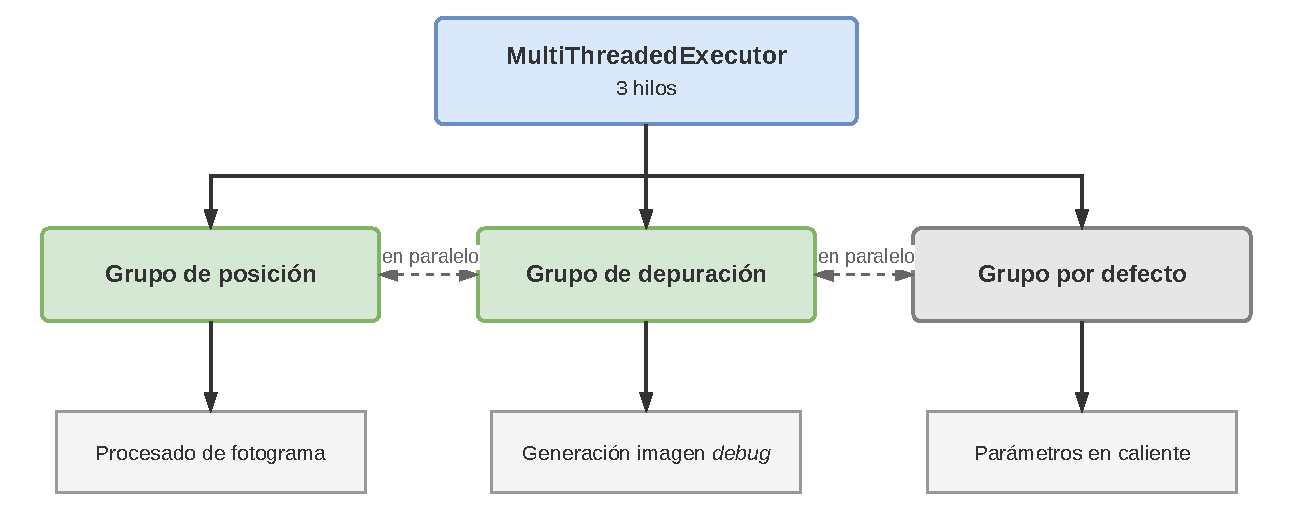
\includegraphics[width=\textwidth]{imaxes/IMPLEMENTACION/multithread_nodo_camara.pdf}
%    \caption{Esquema que permite ver el nivel de concurrencia a nivel de nodo dentro del nodo camara}
%    \label{fig:executor-multihilo}
%\end{figure}
%
%Para optimizar el tener que buscar dentro de un fotograma varios coches implica utilizar también un patrón de concurrencia. En este caso se eligió el patrón productor-consumidor, \ref{fig:modelo-hilos-camara}. El  hilo consumidor coge los fotogramas que la camara recibe cada \qty{33}{\milli\second}, equivalente a la frecuencia máxima de captura de las cámaras empleadas. Después el hilo consumidor se implementa usando un \emph{timer} de ROS2 que coge el último fotograma y lanza su procesamiento sobre un \emph{ThreadPool} con un trabajador por coche: como la búsqueda de cada coche es independiente de las demás, todas se ejecutan concurrentemente sobre el mismo fotograma y el consumidor espera a que terminen antes de darlo por procesado. Se usa un \emph{flag} que impide que un nuevo disparo se solape con un procesamiento en curso. Si el análisis se prolonga, los disparos intermedios se descartan en lugar de encolarse.
%
%\begin{figure}[H]
%    \centering
%    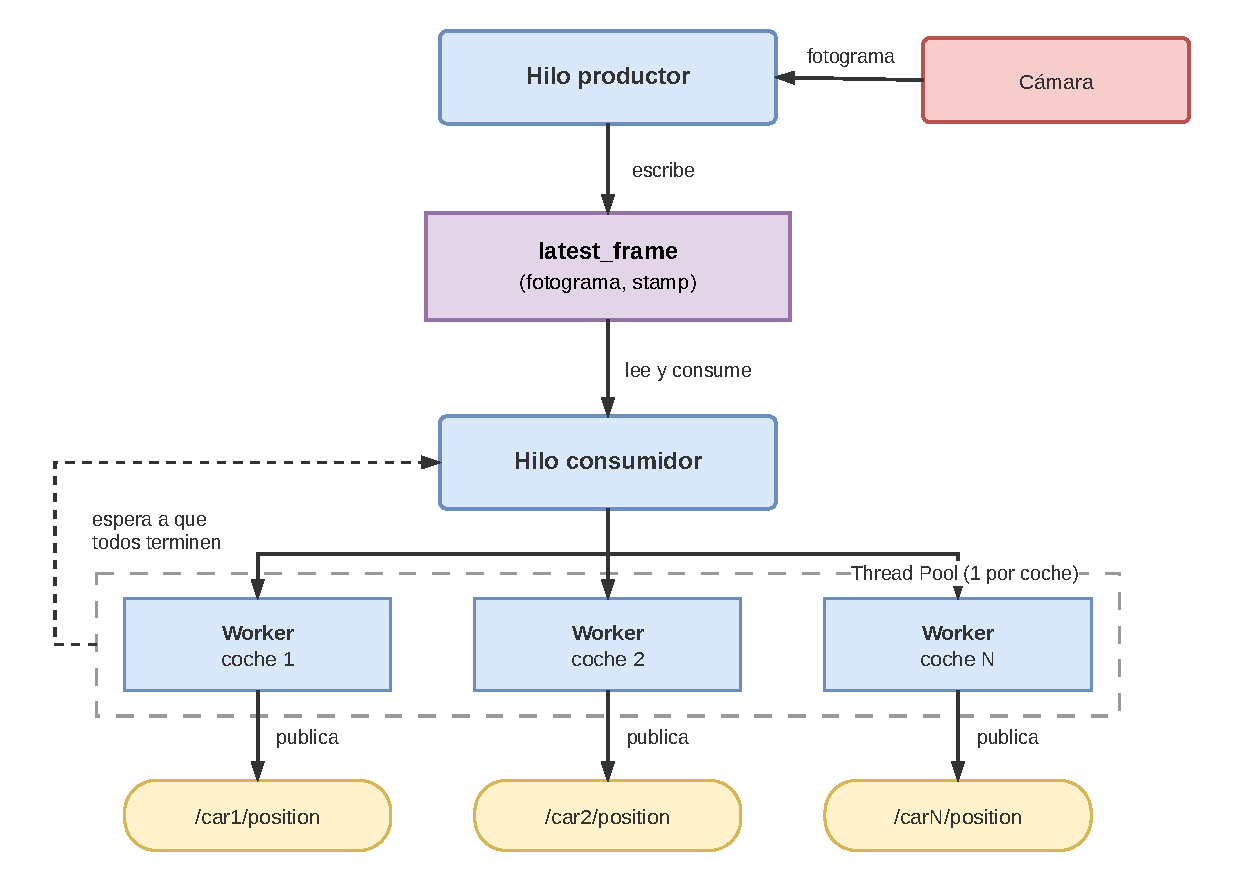
\includegraphics[width=0.75\textwidth]{imaxes/IMPLEMENTACION/productor_consumidor_nodo_camara.pdf}
%    \caption{Modelo de ejecución multihilo productor-consumidor utilizado dentro
%             del nodo de cámara.}
%    \label{fig:modelo-hilos-camara}
%\end{figure}
%
%\subsection{Nodo de control de carril}
%\label{subsec:concurrencia-controlador}
%
%El controlador solo necesita concurrencia a nivel de nodo. Recibe tres \emph{callbacks} distintos: la posición del coche, la orden de cambio de modo y la línea de meta. Como los tres modifican el mismo estado interno, se asignan a un único grupo, el estado del algoritmo queda de este modo en manos de un solo hilo a la vez. Junto a él se conserva el grupo por defecto de ROS~2, atendido por un segundo hilo, que deja disponible la actualización de parámetros en caliente sin interrumpir el control (figura~\ref{fig:concurrencia-controlador}).
%
%\begin{figure}[H]
%    \centering
%    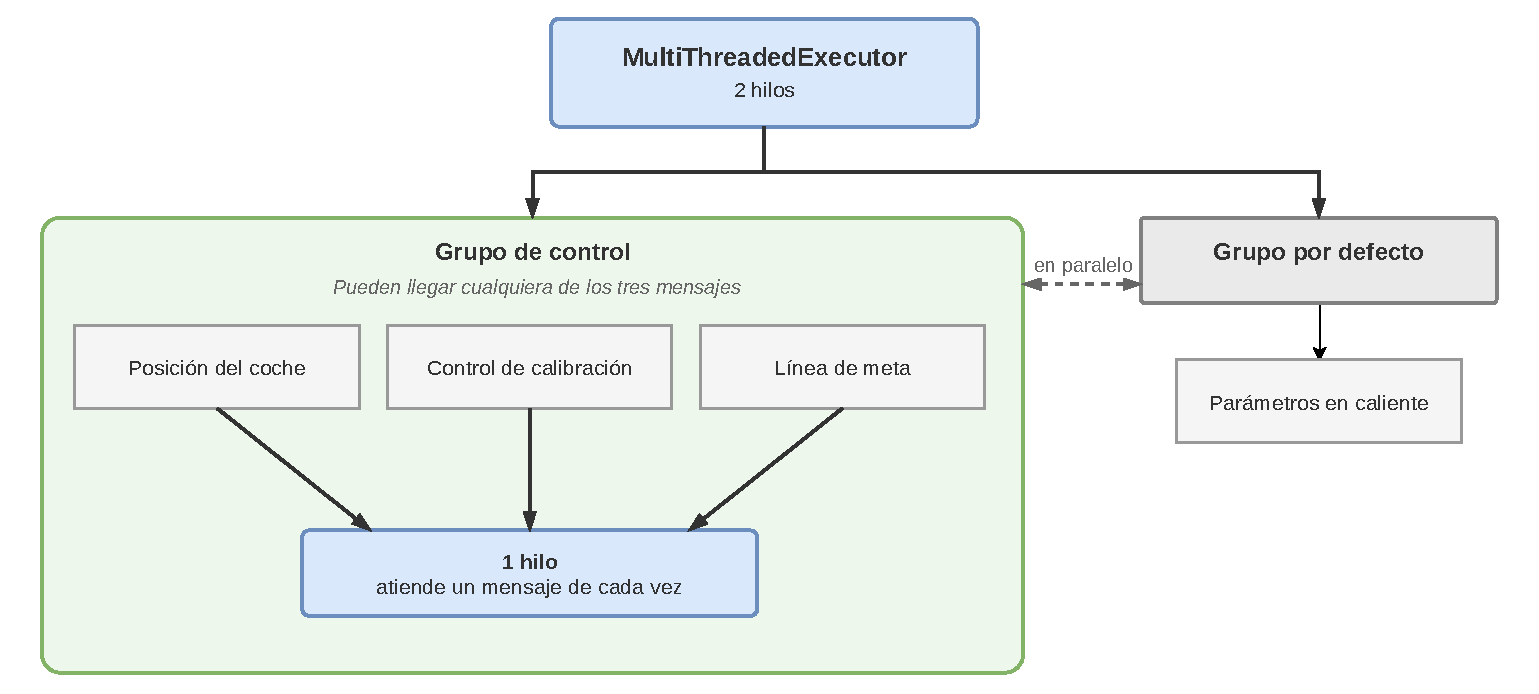
\includegraphics[width=\textwidth]{imaxes/IMPLEMENTACION/multithread_nodo_controlador.pdf}
%    \caption{Modelo de ejecución multihilo a nivel de nodo utilizado dentro del nodo de control de rail}
%    \label{fig:concurrencia-controlador}
%\end{figure}
%
%\subsection{Nodo de actuación}
%\label{subsec:concurrencia-puente}
%
%El puente crea un grupo por cada controlador desplegado, ya que cada uno publica en su propio \emph{topic}, más un grupo para las suscripciones de calibración y el grupo por defecto (figura~\ref{fig:concurrencia-puente}). Así, si el mensaje de un carril se demora no impide recibir y tratar los del resto.
%
%Esta concurrencia en la recepción no puede trasladarse al envío. Existe un único Arduino y un único puerto serie, de modo que el acceso al hardware está necesariamente serializado. La serialización la impone la propia interfaz de comunicación (sección~\ref{subsec:actuacion-interfaz}).
%
%\begin{figure}[H]
%    \centering
%    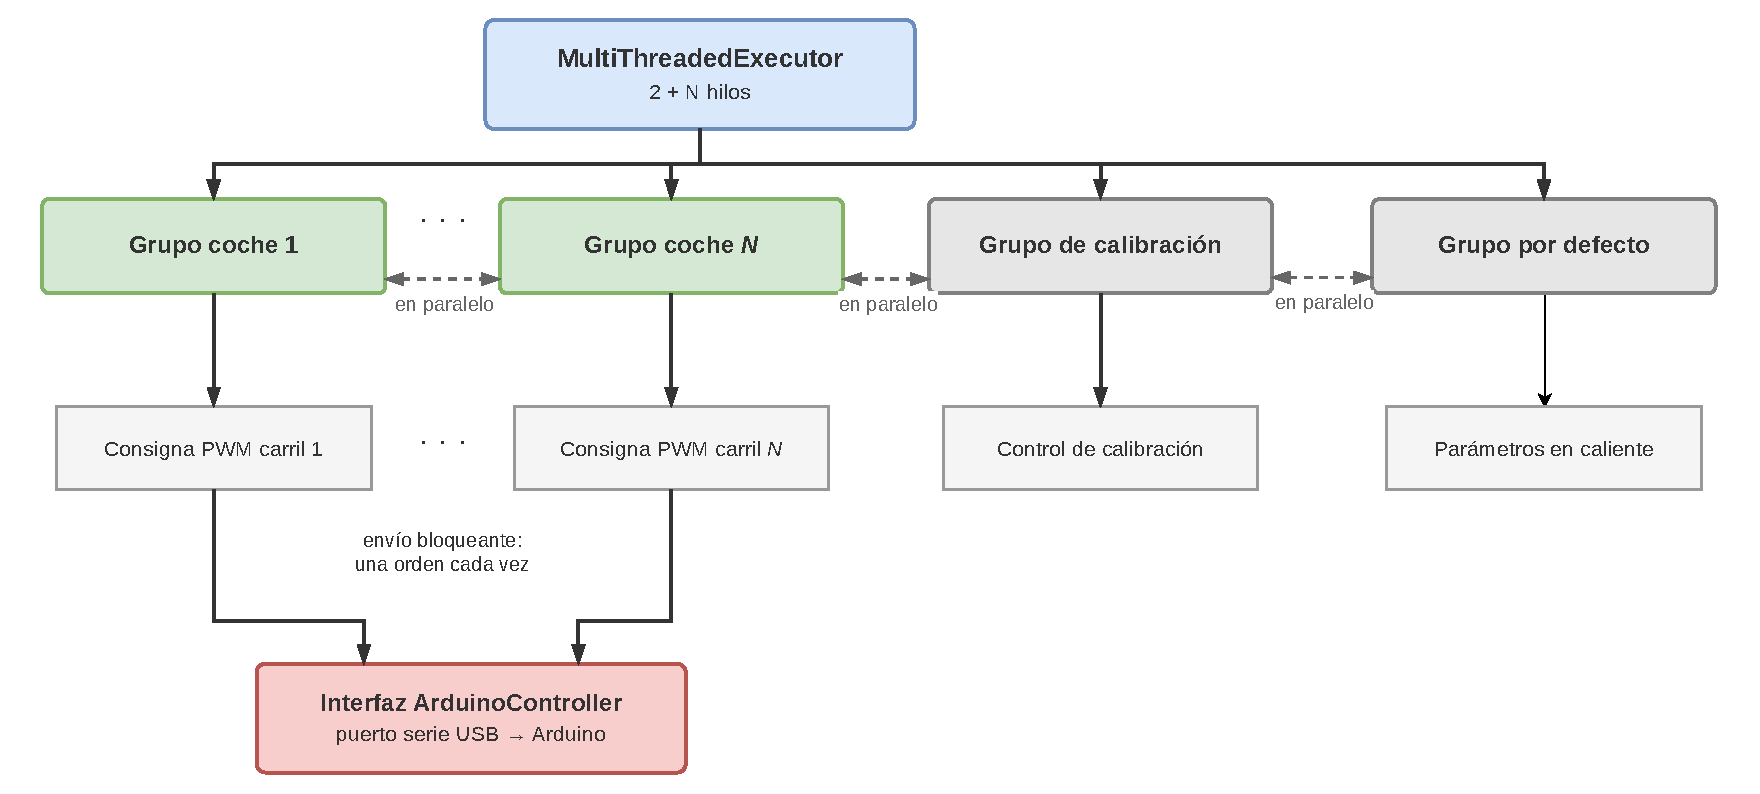
\includegraphics[width=0.9\textwidth]{imaxes/IMPLEMENTACION/multithread_nodo_puente.pdf}
%    \caption{Modelo de ejecución multihilo a nivel de nodo utilizado dentro del nodo puente}
%    \label{fig:concurrencia-puente}
%\end{figure}
%
%\section{Nodo de captura y detección}
%\label{sec:nodo-camara}
%
%El nodo de captura (sección~\ref{sec:arquitectura}) se divide en dos componentes: el nodo de ROS~2, que gestiona la comunicación y los modos de funcionamiento, y un objeto que encapsula la operaciones de visión artificial con las que se obtiene el centroide de cada pegatina. Logrando desacoplar el procesamiento de imagen de la comunicación.
%
%\subsection{Detección de las pegatinas por color}
%\label{subsec:deteccion-etiquetas}
%
%\begin{figure}[H]
%    \centering
%    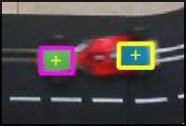
\includegraphics[width=0.6\textwidth]{imaxes/IMPLEMENTACION/deteccion_2_pegatinas.png}
%    \caption{Ejemplo de detección de las dos pegatinas del coche}
%    \label{fig:deteccion-2-pegatinas}
%\end{figure}
%
%La detección hereda el procedimiento del trabajo de Mario López~\cite{tfgmario}. El fotograma se convierte al espacio HSV, que resiste mejor las variaciones de iluminación, y se genera una máscara binaria por pegatina con los píxeles que caen dentro del rango de su color. Están predefinidos para cada uno de los siete colores admitidos. Sobre cada máscara se encadenan una apertura morfológica, que elimina los píxeles aislados, y un cierre morfológico, que rellena los huecos de las regiones válidas.
%
%Se extraen entonces los contornos externos y se toma el de mayor área, descartándolo si no supera un área mínima configurable. De este proceso se obtiene el rectángulo delimitador y el centroide de la pegatina, el significado para cada pegatina se describió en la sección~\ref{sec:arquitectura}. La figura~\ref{fig:deteccion-color} recorre estas etapas sobre un fotograma real.
%
%\begin{figure}[tbp]
%    \centering
%    \begin{subfigure}[b]{0.48\textwidth}
%        \centering
%        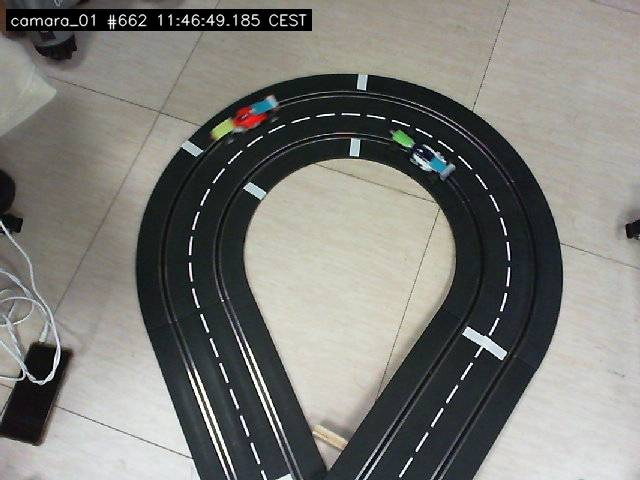
\includegraphics[width=\textwidth]{imaxes/IMPLEMENTACION/det_color_a_original.png}
%        \caption{Fotograma capturado por la cámara}
%        \label{fig:deteccion-color-a}
%    \end{subfigure}
%    \hfill
%    \begin{subfigure}[b]{0.48\textwidth}
%        \centering
%        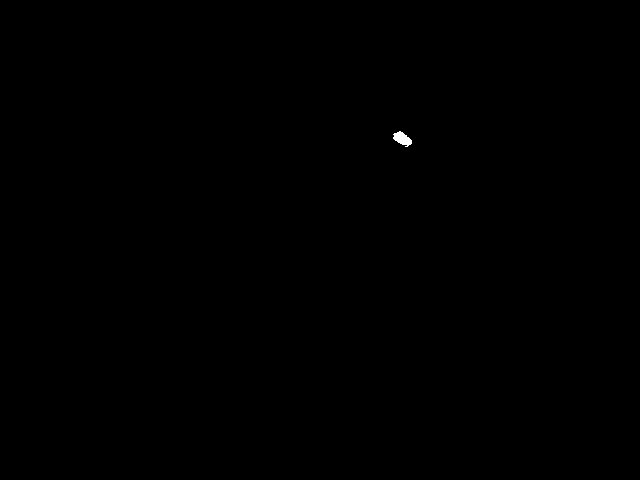
\includegraphics[width=\textwidth]{imaxes/IMPLEMENTACION/det_color_b_mascara.png}
%        \caption{Máscara del color de la pegatina verde delantera del coche azul}
%        \label{fig:deteccion-color-b}
%    \end{subfigure}
%
%    \vspace{0.7em}
%    \begin{subfigure}[b]{0.34\textwidth}
%        \centering
%        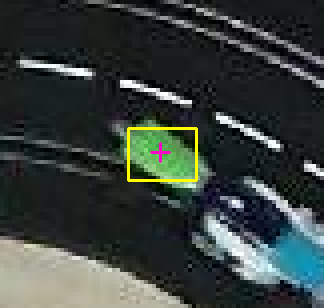
\includegraphics[width=\textwidth]{imaxes/IMPLEMENTACION/det_color_c_resultado.png}
%        \caption{Rectángulo y centroide detectados después de realizar las operaciones pertinentes}
%        \label{fig:deteccion-color-c}
%    \end{subfigure}
%    \caption{Ejemplo del proceso de detección que realiza el nodo camara para detectar una de las pegatinas del coche}
%    \label{fig:deteccion-color}
%\end{figure}
%
%\subsection{Diferencias entre calibración y carrera}
%\label{subsec:modos-funcionamiento}
%
%El nodo implementa los dos modos descritos en la sección~\ref{sec:modos_funcionamiento}, y la diferencia entre ambos está en la región del fotograma sobre la que busca.
%
%En calibración, cada detección de la pegatina delantera se añade a la lista que reconstruye la trayectoria del coche. Basta con la delantera, que es la que da una trayectoria limpia~\cite{tfgadrian}. Esto es porque la trasera puede quedar oculta a ratos y la ruta base debe registrarse sin interrupciones. Al mantener una trayectoria por coche, la cámara puede filtrar por carril en carrera y dos coches pueden compartir el color de la pegatina trasera. Durante todo este proceso se busca sobre el fotograma completo como el que se puede ver \ref{fig:deteccion-color-a}, es por ello que las pegatinas delanteras sí que tienen que ser de diferente color.
%
%La calibración termina por coche, no para todo el sistema. El nodo se suscribe al \emph{topic} de calibración de cada coche configurado y, al recibir el aviso de que uno ha completado su vuelta, genera su máscara con los puntos acumulados. Desde ese momento la búsqueda de ese coche queda restringida a una franja alrededor del recorrido conocido, como recoge la figura~\ref{fig:mascara-trayectoria}.
%
%\begin{figure}[tbp]
%    \centering
%    \begin{subfigure}[b]{0.32\textwidth}
%        \centering
%        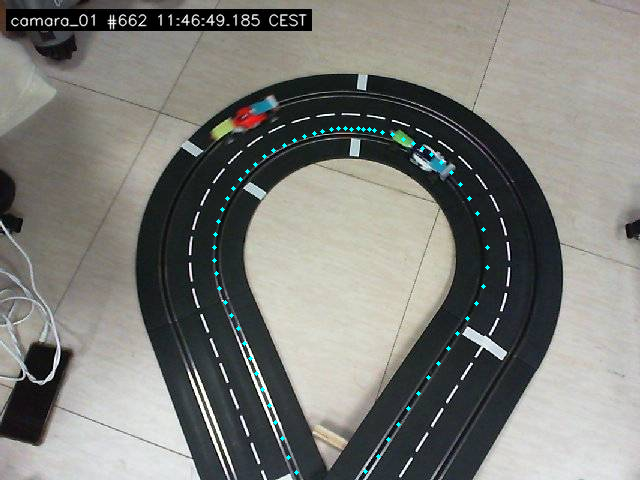
\includegraphics[width=\textwidth]{imaxes/IMPLEMENTACION/mascara_a_puntos.png}
%        \caption{Posiciones acumuladas durante la vuelta de calibración}
%        \label{fig:mascara-trayectoria-a}
%    \end{subfigure}
%    \hfill
%    \begin{subfigure}[b]{0.32\textwidth}
%        \centering
%        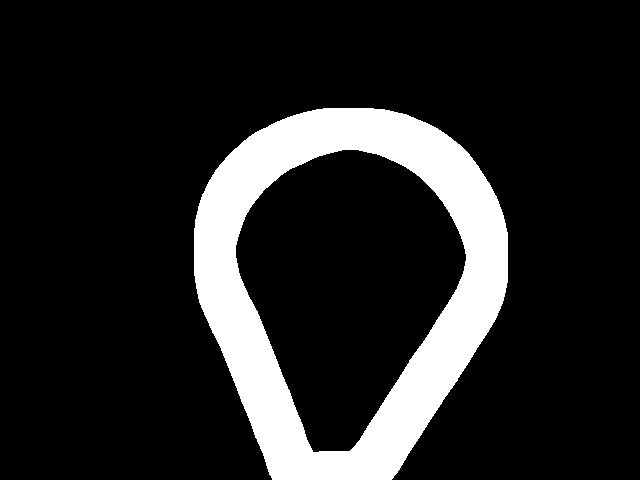
\includegraphics[width=\textwidth]{imaxes/IMPLEMENTACION/mascara_b_mascara.png}
%        \caption{Máscara generada a partir de la posición que sigue el coche}
%        \label{fig:mascara-trayectoria-b}
%    \end{subfigure}
%    \hfill
%    \begin{subfigure}[b]{0.32\textwidth}
%        \centering
%        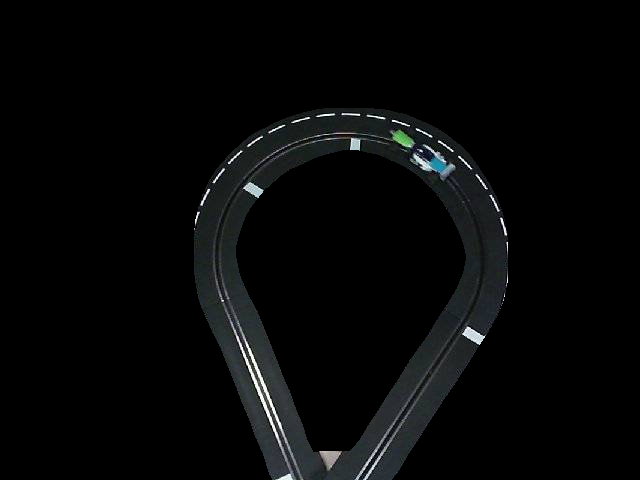
\includegraphics[width=\textwidth]{imaxes/IMPLEMENTACION/mascara_c_filtrado.png}
%        \caption{Fotograma filtrado después de aplicar la mascara generada durante la calibración}
%        \label{fig:mascara-trayectoria-c}
%    \end{subfigure}
%    \caption{Ejemplo de proceso de generación de la máscara de trayectoria para un coche. Deja fuera el carril contrario, con lo que el coche que circula por él deja de ser un falso positivo posible.}
%    \label{fig:mascara-trayectoria}
%\end{figure}
%
%\subsection{Seguimiento mediante región de interés}
%\label{subsec:seguimiento-roi}
%
%En carrera la búsqueda se restringe a una región de interés de $150 \times 150$ píxeles centrada en la posición predicha para el coche. La predicción es la extrapolación lineal que introdujo Mario López~\cite{tfgmario}. Conocidas las dos últimas posiciones, el centro de la región es la actual más el vector de movimiento del último fotograma.
%
%Sobre ella se aplica además la máscara de trayectoria, de modo que solo sobreviven los píxeles que pertenecen a la vez a la región y a las proximidades del carril; la intersección de ambos filtros procede también de los trabajos previos~\cite{tfgmario,tfgadrian}. La detección de las pegatinas (\ref{subsec:deteccion-etiquetas}) se realiza sobre esa imagen reducida, se puede ver un ejemplo en \ref{fig:roi-filtrado}. El problema que presenta hacerlo de esta manera es que sus coordenadas son relativas a la región y hay que trasladarlas al sistema de referencia de la cámara antes de publicarlas.
%
%\begin{figure}[tbp]
%    \centering
%    \begin{subfigure}[b]{0.55\textwidth}
%        \centering
%        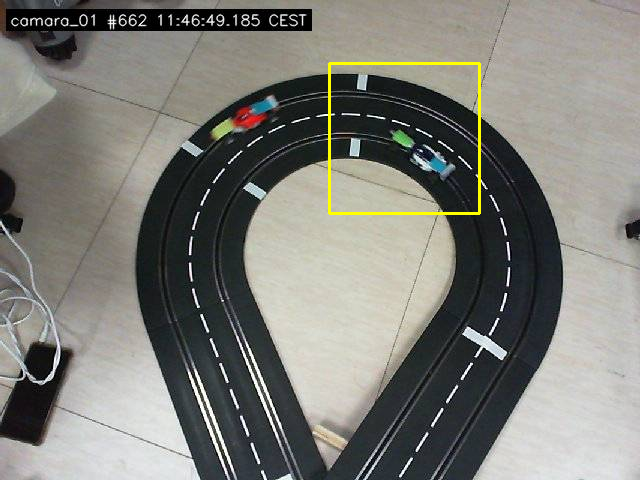
\includegraphics[width=\textwidth]{imaxes/IMPLEMENTACION/roi_a_recuadro.png}
%        \caption{Región de interés marcada sobre todo el fotograma}
%        \label{fig:roi-filtrado-a}
%    \end{subfigure}
%    \hfill
%    \begin{subfigure}[b]{0.38\textwidth}
%        \centering
%        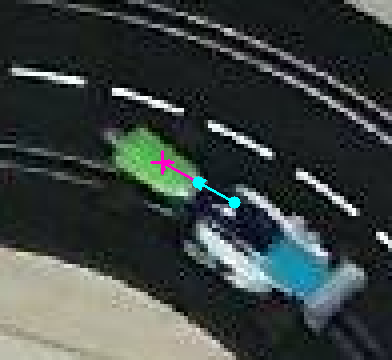
\includegraphics[width=\textwidth]{imaxes/IMPLEMENTACION/roi_b_extrapolacion.png}
%        \caption{Extrapolación de la posición}
%        \label{fig:roi-filtrado-b}
%    \end{subfigure}
%
%    \vspace{0.7em}
%    \begin{subfigure}[b]{0.32\textwidth}
%        \centering
%        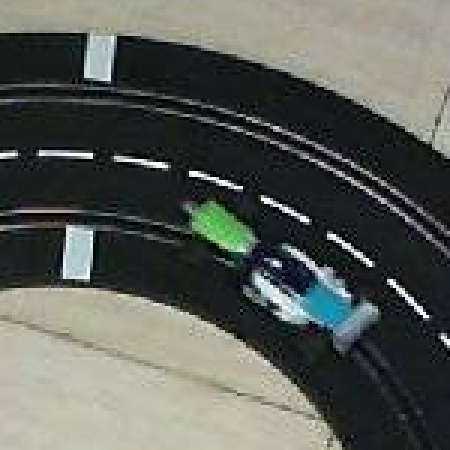
\includegraphics[width=\textwidth]{imaxes/IMPLEMENTACION/roi_c_recorte.png}
%        \caption{Recorte de la región}
%        \label{fig:roi-filtrado-c}
%    \end{subfigure}
%    \hspace{0.04\textwidth}
%    \begin{subfigure}[b]{0.32\textwidth}
%        \centering
%        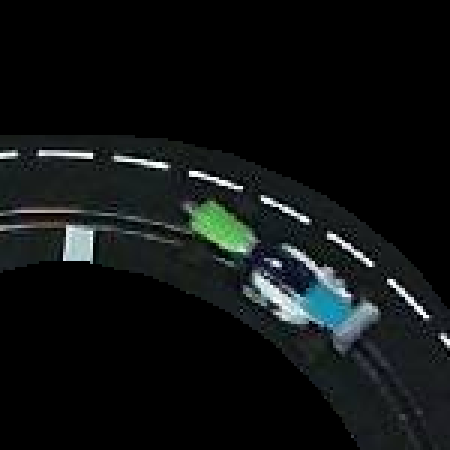
\includegraphics[width=\textwidth]{imaxes/IMPLEMENTACION/roi_d_filtrado.png}
%        \caption{Región tras la intersección entre la mascara y el ROI}
%        \label{fig:roi-filtrado-d}
%    \end{subfigure}
%    \caption{Explicación del proceso de obtención del ROI y aplicación dentro del sistema. En el detalle, las dos flechas encadenadas son el desplazamiento medido entre los dos últimos fotogramas. La cruz marca la posición predicha, que en este fotograma cae a 1,6 píxeles de la real. El último panel es lo único que llega al detector de color.}
%    \label{fig:roi-filtrado}
%\end{figure}
%
%\subsection{Readquisición del seguimiento}
%\label{subsec:readquisicion}
%
%Las oclusiones son habituales en un circuito de Scalextric~\cite{tfgmario}, y un derrape brusco puede alejar el coche de la posición predicha. En ambos casos la detección fracasa y hay que recuperar el seguimiento.
%
%La estrategia es ampliar progresivamente la zona de búsqueda. Cada fotograma sin detección incrementa el tamaño de la región en 50 píxeles, hasta abarcar como máximo la imagen completa. Los trabajos previos pasaban de golpe a examinar toda la proximidad de la trayectoria; el crecimiento gradual acota el coste de los fotogramas inmediatamente posteriores a la pérdida.
%
%Al perder el seguimiento se descartan las posiciones anteriores, como ya hacía Mario López~\cite{tfgmario}, para que la extrapolación no combine un punto previo a la pérdida con el primero posterior y sitúe la región lejos del coche. La primera detección tras readquirir centra la región sobre la posición encontrada.
%
%\subsection{Detección de la línea de meta}
%\label{subsec:deteccion-meta}
%
%La línea de meta se señaliza con una etiqueta alargada de un color reservado que atraviesa la pista. Se detecta una sola vez, al arrancar el nodo, porque su posición no cambia durante la carrera.
%
%El procedimiento empleado para la detección de la línea de meta es el de Adrián Rego~\cite{tfgadrian}. Al igual que en la detección de las pegatinas, el fotograma se convierte al espacio de color HSV y se genera una máscara binaria con el rango del color reservado para la meta (se puede cambiar desde el fichero de configuración \ref{subsec:params-yaml}), de forma que se genera una mascara binaria con los píxeles de la etiqueta. Sobre está se aplica un cierre morfólogico con un tamaño de \emph{kernel} muy grande, porque los raíles y las ranuras de la pista atraviesan la etiqueta y la fragmentan en trozos que hay que unir en una única región. Sobre está región se calcula el rectángulo de área mínima que lo encierra, el cual, a diferencia del rectángulo delimitador convencional, puede estar rotado y se adapta así a la orientación real de la linea de meta. De sus cuatro vértices se identifican los dos lados cortos comparando las longitudes de las aristas adyacentes, y el segmento que une sus puntos medios define la línea de meta. La figura~\ref{fig:deteccion-meta} muestra las tres etapas del proceso.
%
%\begin{figure}[tbp]
%    \centering
%    \begin{subfigure}[b]{0.32\textwidth}
%        \centering
%        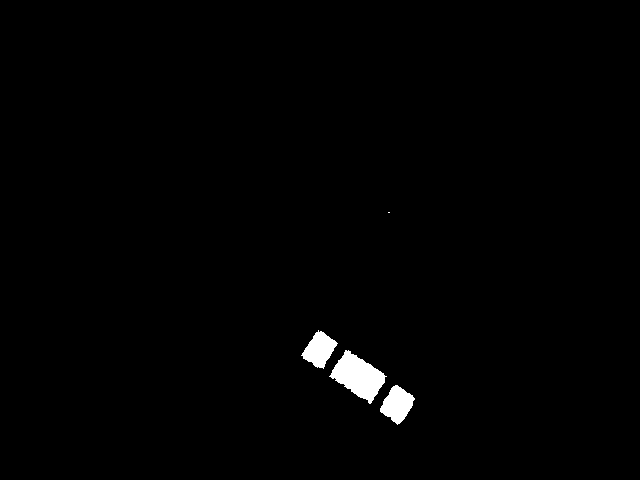
\includegraphics[width=\textwidth]{imaxes/IMPLEMENTACION/meta_a_mascara.png}
%        \caption{Máscara del color de la meta}
%        \label{fig:deteccion-meta-a}
%    \end{subfigure}
%    \hfill
%    \begin{subfigure}[b]{0.32\textwidth}
%        \centering
%        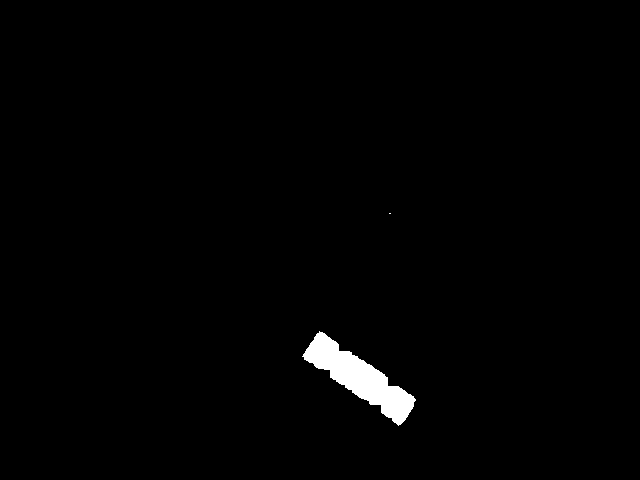
\includegraphics[width=\textwidth]{imaxes/IMPLEMENTACION/meta_b_cierre.png}
%        \caption{Tras el cierre morfológico}
%        \label{fig:deteccion-meta-b}
%    \end{subfigure}
%    \hfill
%    \begin{subfigure}[b]{0.32\textwidth}
%        \centering
%        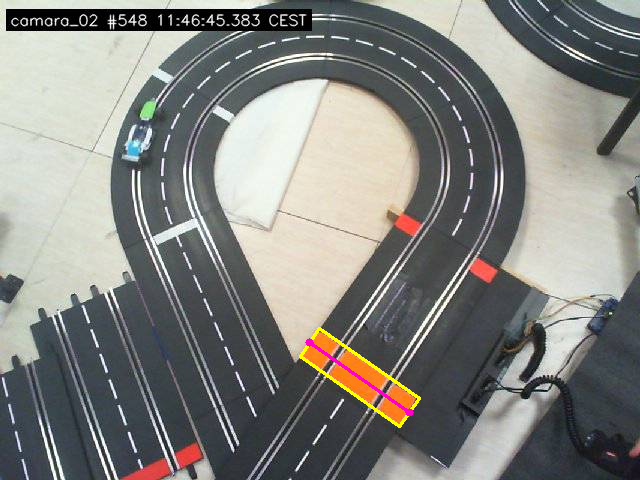
\includegraphics[width=\textwidth]{imaxes/IMPLEMENTACION/meta_c_segmento.png}
%        \caption{Rectángulo y segmento}
%        \label{fig:deteccion-meta-c}
%    \end{subfigure}
%    \caption{Detección de la línea de meta en la cámara~2. Los raíles parten la etiqueta en tres trozos que el cierre morfológico vuelve a unir; sobre la región resultante se ajusta el rectángulo de área mínima, rotado, y los puntos medios de sus lados cortos dan el segmento de meta.}
%    \label{fig:deteccion-meta}
%\end{figure}
%
%Cada nodo la busca al arrancar y, si no la ve, no publica línea de meta alguna. Por lo que en un despliegue multicámara solo lo hace la que observa la linea y generando el mensaje correspondiente (cuadro~\ref{tab:mensajes}). No hay, por tanto, una cámara de meta designada de antemano por el usuario.
%
%\subsection{Modo de depuración}
%\label{subsec:modo-depuracion}
%
%El nodo ofrece un modo de depuración, desactivado por defecto y activable en caliente o desde el fichero de parametros \ref{subsec:params-yaml}. En caso de que el flag este activado se conserva una copia del fotograma procesado sobre el cual se dibujan los rectángulos delimitadores de las pegatinas y una cruceta sobre cada centroide, y en una esquina su se pone el identificador del nodo, el número de fotograma y la hora de captura. El resultado se publica como \emph{vista de la cámara} (sección~\ref{subsec:mensajes-propios}), que es lo que permite seguir cada cámara en directo y lo que graba el sistema de visualización.
%
%\section{Nodo de control de carril}
%\label{sec:control-rail}
%
%El nodo controlador, uno por raíl según la sección~\ref{sec:arquitectura}, se divide como el de captura en dos componentes: el nodo de ROS~2, que gestiona la comunicación, los modos de funcionamiento y la detección del paso por meta, y un objeto que encapsula el algoritmo de velocidad, cuya implementación se detalla en la sección~\ref{sec:implementacion-algoritmo}.
%
%\subsection{Construcción de la trayectoria base}
%\label{subsec:control-modos}
%
%El nodo implementa los dos modos descritos en la sección~\ref{sec:modos_funcionamiento}, y su comportamiento cambia por completo de uno a otro.
%
%Durante la calibración el controlador acumula la posición de la pegatina delantera en un diccionario indexado por cámara: cada nodo de captura del que recibe mensajes tiene su propia lista de puntos y en ningún momento se construye una lista única con el circuito completo. Lo que delimita la acumulación es el paso por meta. Los puntos se recogen entre el primer cruce y el segundo, de modo que cada trayectoria base es una única vuelta que empieza en la meta; todo lo anterior, colocar el coche, arrancarlo y las vueltas que dé mientras se levanta el sistema, se descarta. El nodo sabe por sí solo cuándo terminar, porque es él quien detecta el paso por meta de su coche (sección~\ref{subsec:control-meta}).
%
%Al cerrarse la vuelta el controlador lo notifica en su \emph{topic} de calibración, filtra cada lista descartando los puntos que queden a menos de un umbral configurable del último aceptado, crea una instancia del algoritmo por cada cámara del diccionario, le inyecta su trayectoria y guarda una copia en la caché de la sección~\ref{subsec:cache-calibracion}.
%	
%Que se cierre sola es un requisito de la arquitectura. En los trabajos previos la arrancaba y la daba por concluida una persona desde una interfaz gráfica: había que delimitar el coche con un rectángulo y marcar la meta a mano~\cite{tfgmario}, o seleccionar el vehículo, activar el modo de búsqueda y confirmar los valores obtenidos~\cite{tfgadrian}. Con los nodos repartidos entre varias máquinas y sin interfaz desde la que supervisarlos, la calibración tiene que delimitarse y terminarse con la información que ya circula por la red.
%
%En modo carrera el controlador deja de acumular puntos y pasa a enrutar. Cada mensaje de posición de su coche se entrega a la instancia del algoritmo de la cámara que lo originó, identificada por el campo \texttt{camara\_id} del mensaje (sección~\ref{subsec:mensajes-propios}). La instancia devuelve el valor de PWM que hay que aplicar, que el controlador publica en su \emph{topic} de consigna, o bien la indicación de descartar el fotograma, en cuyo caso se mantiene el último valor válido. El funcionamiento interno del algoritmo se detalla en la sección~\ref{sec:implementacion-algoritmo}.
%
%Si se ordena volver al modo calibración, se descartan las trayectorias y las instancias y el proceso empieza de cero.
%
%\subsection{Control automático y control manual}
%\label{subsec:control-automatico-manual}
%
%Cerrada la calibración, el controlador entra en modo carrera y pasa de acumular puntos a enrutar posiciones. Es la pieza del sistema que aplica el algoritmo de velocidad, y cómo lo hace depende del indicador \texttt{modo\_manual} del coche, que se declara en el fichero de parámetros (sección~\ref{subsec:params-yaml}) y determina desde qué fichero de lanzamiento se levanta el nodo (sección~\ref{subsec:launch-files}).
%
%En control automático, cada mensaje de posición de su coche se entrega a la instancia del algoritmo de la cámara que lo originó, identificada por el campo \texttt{camara\_id} del mensaje (sección~\ref{subsec:mensajes-propios}). La instancia devuelve el valor de PWM que hay que aplicar, que el controlador publica en su \emph{topic} de consigna para que lo recoja el nodo puente, o bien la indicación de descartar el fotograma, en cuyo caso se mantiene el último valor válido. El controlador no decide nada por su cuenta: toda la lógica de control reside en el algoritmo, cuya implementación se detalla en la sección~\ref{sec:implementacion-algoritmo}.
%
%En control manual conduce una persona con el mando y el controlador no publica consigna alguna, de modo que el nodo puente nunca toca ese carril (sección~\ref{subsec:actuacion-topics}). El nodo hace por lo demás el mismo trabajo: calibra, sigue recibiendo posiciones, cuenta las vueltas de su coche y publica su telemetría. Sirve para registrar una carrera conducida por una persona con el mismo formato de datos que una automática, de manera que ambas puedan compararse después con la herramienta de análisis (sección~\ref{subsec:visualizacion-analisis}).
%
%Una carrera mixta, con coches de los dos tipos, se consigue levantando a la vez los dos ficheros de lanzamiento, tal como se describe en la sección~\ref{subsec:launch-files}.
%
%\subsection{Detección del paso por meta y medición de tiempos}
%\label{subsec:control-meta}
%
%El controlador cuenta las vueltas de su coche y mide su duración, que es lo que cierra el ciclo de aprendizaje del algoritmo (sección~\ref{subsec:algoritmo-aprendizaje}).
%
%El mecanismo se hereda del trabajo de Mario López~\cite{tfgmario} y solo se aplica a los mensajes de la cámara que publicó la línea de meta. Para cada posición se calcula el producto vectorial entre el vector que recorre el segmento de meta y el que va de uno de sus extremos a la pegatina delantera. Su signo indica de qué lado de la recta que contiene al segmento está el coche, de modo que un cambio de signo entre dos fotogramas consecutivos significa que lo ha cruzado.
%
%\begin{figure}[tbp]
%    \centering
%    \begin{subfigure}[b]{0.48\textwidth}
%        \centering
%        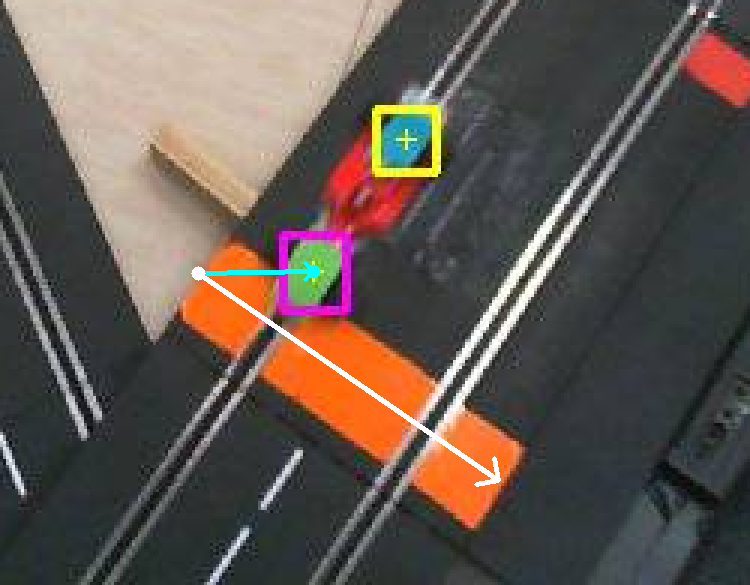
\includegraphics[width=\textwidth]{imaxes/IMPLEMENTACION/meta_vector_a_antes.png}
%        \caption{Antes de cruzar}
%        \label{fig:producto-vectorial-a}
%    \end{subfigure}
%    \hfill
%    \begin{subfigure}[b]{0.48\textwidth}
%        \centering
%        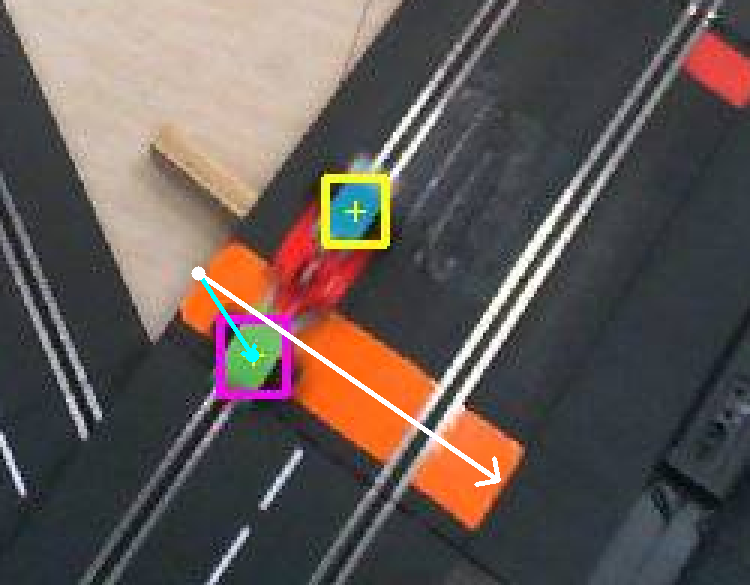
\includegraphics[width=\textwidth]{imaxes/IMPLEMENTACION/meta_vector_b_despues.png}
%        \caption{Después de cruzar}
%        \label{fig:producto-vectorial-b}
%    \end{subfigure}
%    \caption{Ejemplo de cómo se detecta el cruce por meta}
%    \label{fig:producto-vectorial}
%\end{figure}
%
%Detectado el cambio de lado, el instante del cruce se aproxima interpolando entre los dos fotogramas implicados, el anterior a la meta y el posterior. La fracción del intervalo recorrida hasta tocar la recta es el cociente entre la distancia del fotograma anterior y la suma de ambas distancias. Sin interpolar, tomar la marca del fotograma que detecta el cruce introduciría un error de hasta un período de captura en cada vuelta.
%
%Los instantes que se interpolan son las marcas de tiempo que la cámara pone al capturar el fotograma, no el momento en que llega el mensaje, por la razón expuesta en la sección~\ref{subsec:qos}. Así no hace falta sincronizar los relojes de las máquinas, porque el tiempo por vuelta se calcula siempre contra la misma referencia temporal, la de la cámara. En cada cruce el controlador publica el tiempo y el número de vuelta en su \emph{topic} de telemetría y notifica el evento a todas las instancias del algoritmo, indicando si la vuelta fue limpia.
%
%El método arrastra una limitación que ya señalaba Mario López~\cite{tfgmario}: el signo se calcula contra la recta infinita que contiene al segmento y, como el circuito es cerrado, esa recta vuelve a cortar la pista en otro punto, donde el signo cambia igual. Él lo evitaba calculando el producto solo con el coche a menos de vez y media su longitud de un extremo de la meta; aquí el cambio de signo se ignora mientras la distancia de la pegatina a la meta supere un umbral configurable.
%
%% TODO: figura de la recta de meta prolongada cortando el circuito en un segundo punto (equivalente a la figura 5.9 de la memoria de Mario López)
%
%Este método sustituye al del trabajo de Adrián Rego~\cite{tfgadrian}, que fue el primero que se implementó. Con el coche muy lento o detenido sobre la línea de meta llegaba a fallar la cuenta, de modo que se cambió por el del cambio de signo, que no depende de la velocidad a la que se cruce.
%
%\section{Implementación del algoritmo de velocidad}
%\label{sec:implementacion-algoritmo}
%
%Esta sección detalla cómo se implementa el algoritmo cuyo diseño se describió en la sección~\ref{sec:algoritmo-arquitectura}. Su entrada es una posición del coche sobre la imagen de una cámara y su salida el valor de PWM que hay que aplicar al carril. Durante este proceso se usa la trayectoria base aprendida durante la calibración, se detectan derrapes y se aplican las dos políticas de ajuste.
%
%\subsection{Instancias por cámara}
%\label{subsec:algoritmo-instancias}
%
%El algoritmo no trabaja sobre el circuito completo, sino sobre la porción que observa una cámara. El controlador mantiene un diccionario indexado por identificador de cámara (sección~\ref{subsec:control-modos}), que guarda la lista de puntos acumulados de esa cámara durante la calibración. Al cerrarse la vuelta, cada lista da lugar a una instancia independiente del algoritmo, con su propia cadena de celdas, sus propias zonas y su propio perfil de PWM.
%
%La consecuencia es que no existe una trayectoria global del circuito. Cada trayectoria vive en las coordenadas de imagen de su cámara y ninguna instancia conoce nada de las demás, no hay fusión de trayectorias y  tampoco un sistema de referencia común. El único punto del proyecto en el que todas se llevan a un plano común es la herramienta de análisis en diferido (sección~\ref{subsec:visualizacion-analisis}), que queda fuera del lazo de control. Hacerlo de esta forma es porque permite facilita el trabajo y reduce el esfuerzo que hay que realizar.
%
%La visión de conjunto la aporta el controlador, no el algoritmo. Es el controlador quien enruta cada posición a la instancia que le corresponde, quien decide qué cámara está activa en cada momento, quien cierra un derrape en una cámara y abre su continuación en la siguiente, quien propaga hacia atrás las reducciones que no caben en una porción y quien determina si una vuelta ha sido limpia en todo el trazado. Esos mecanismos se describen en la sección~\ref{subsec:algoritmo-coordinacion}.
%
%\subsection{Construcción de la cadena de celdas}
%\label{subsec:algoritmo-celdas}
%
%La trayectoria base de la sección~\ref{subsec:trayectoria-base} se transforma en una sucesión ordenada de celdas. Al terminar la calibración cada instancia recibe la lista de puntos de su cámara y la remuestrea, porque los puntos crudos no están repartidos de forma uniforme, su separación depende de la velocidad que llevase el coche al grabarlos y de si todas las posiciones enviadas por la camara llegaron al controlador. Se recorre esta trayectoria colocando una celda cada cierta distancia fija e interpolando entre puntos consecutivos, de modo que las celdas quedan equiespaciadas sobre la trayectoria real que sigue el coche en el circuito, independientemente de como cayeran los puntos originales. 
%
%Los saltos entre puntos consecutivos que superan un umbral reciben otro tratamiento. Corresponden a tramos que la cámara no ve, porque un puente o otro elemento tapan la pista, y no tiene sentido interpolar dentro de ellos. En su lugar se crea una única \emph{celda gigante} que registra la longitud real del hueco. Dentro de ella no puede localizarse el coche ni detectarse derrapes, pero se trata todo con un mismo valor de PWM.
%
%\subsection{Localización del coche sobre la trayectoria}
%\label{subsec:algoritmo-localizacion}
%
%Para poder realizar el control es necesario saber donde están las dos pegatinas del coche, tanto la delantera como la trasera, con respecto a la trayectoria base, (sección~\ref{subsec:trayectoria-base}). Razón por la cual, para cada una se obtiene la celda más cerca y su distancia a ella.
%
%Después cada una tiene un uso distinto. La distancia de la delantera es una comprobación realizada para comprobar que el coche sigue el recorrido esperado, si supera un umbral se considera que la detección no es válida y el fotograma se descarta sin llegar a calcular un PWM nuevo. La distancia de la trasera es la señal con la que se detectan los derrapes, como se detalla en la sección~\ref{subsec:algoritmo-derrapes}.
%
%El procedimiento es el mismo para ambas. Primero se busca la celda cuyo punto está más próximo al centroide de la pegatina. Después se proyecta ese centroide sobre los dos segmentos que unen la celda escogida con su anterior y su posterior, y se conserva la menor de las dos distancias. La proyección hace falta porque medir contra la celda daría una distancia que no es precisa, en cambio contra los segmentos se obtiene la distancia perpendicular a la trayectoria.
%
%La proyección solo puede hacerse entre celdas consecutivas, porque a través de una celda gigante no hay trayectoria conocida sobre la que proyectar. .
%
%\subsection{Detección de derrapes}
%\label{subsec:algoritmo-derrapes}
%
%La sección~\ref{subsec:derrape-arquitectura} exige que exista una señal capaz de indicar en qué punto del circuito el coche ha perdido el control, es decir, derrapado. La señal escogida aquí es la distancia perpendicular de la pegatina trasera a la trayectoria. Cuando la parte trasera del coche se abre, esa distancia crece, mientras la delantera sigue marcando la posición sobre el trazado.
%
%La detección se implementa como una máquina de estados que se alimenta en cada fotograma con la celda y la distancia perpendicular de la pegatina trasera. Cuando la distancia supera el umbral de derrape se abre uno y se anota la celda inicial, mientras se mantenga por encima, el derrape se prolonga actualizando su celda final; cuando vuelve a caer por debajo, se cierra. No se abren derrapes junto a los extremos de la cadena ni junto a las celdas gigantes, donde la medida no es fiable.
%
%La figura~\ref{fig:secuencia-derrape} ejemplifica un caso donde se puede ver el proceso real de derrape del coche. Con el coche alineado la pegatina trasera va sobre el carril y su distancia a la trayectoria es casi nula; al abrirse la parte trasera la distancia perpendicular del centroide de la pegatina a la trayectoria crece hasta superar el umbral, que es lo que abre el derrape, se puede ver en la figura~\ref{fig:derrape-trazas-b}. En el instante más violento el coche queda atravesado y ninguna de las dos pegatinas se detecta, situación que resuelve la readquisición de la sección~\ref{subsec:readquisicion}.
%
%\begin{figure}[tbp]
%    \centering
%    \begin{subfigure}[b]{0.48\textwidth}
%        \centering
%        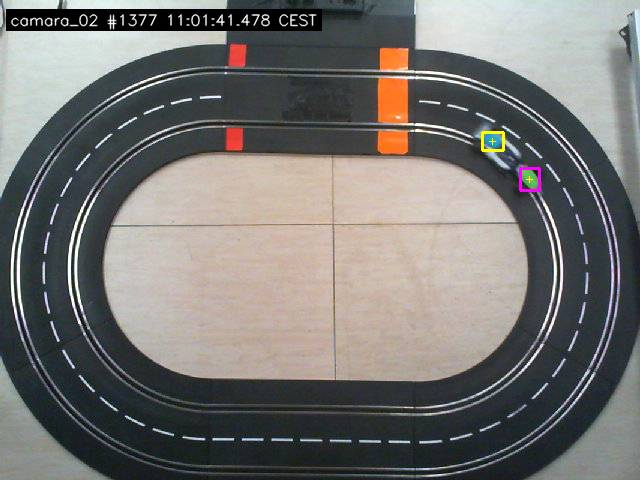
\includegraphics[width=\textwidth]{imaxes/IMPLEMENTACION/derrape_seq_a_antes.png}
%        \caption{Coche alineado con el carril}
%        \label{fig:secuencia-derrape-a}
%    \end{subfigure}
%    \hfill
%    \begin{subfigure}[b]{0.48\textwidth}
%        \centering
%        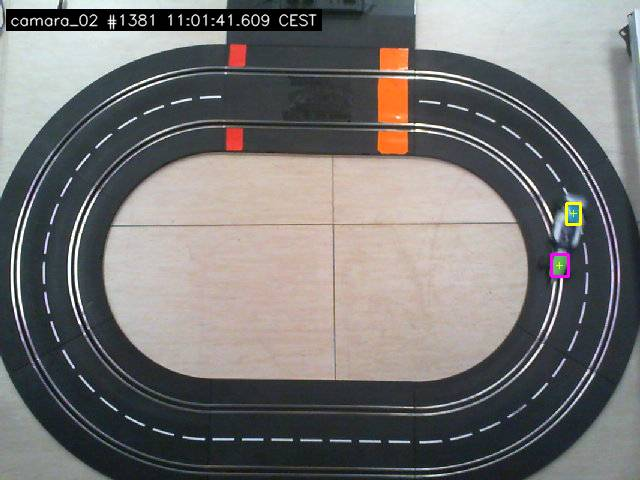
\includegraphics[width=\textwidth]{imaxes/IMPLEMENTACION/derrape_seq_b_inicio.png}
%        \caption{La parte trasera empieza a abrirse}
%        \label{fig:secuencia-derrape-b}
%    \end{subfigure}
%
%    \vspace{0.7em}
%    \begin{subfigure}[b]{0.48\textwidth}
%        \centering
%        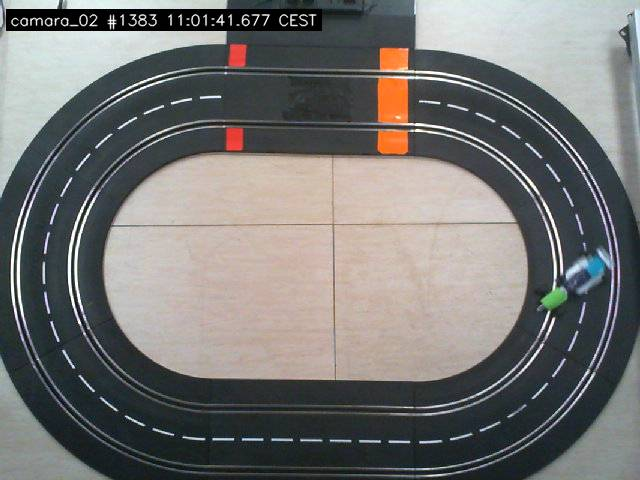
\includegraphics[width=\textwidth]{imaxes/IMPLEMENTACION/derrape_seq_c_completo.png}
%        \caption{Derrape completo, sin detección}
%        \label{fig:secuencia-derrape-c}
%    \end{subfigure}
%    \hfill
%    \begin{subfigure}[b]{0.48\textwidth}
%        \centering
%        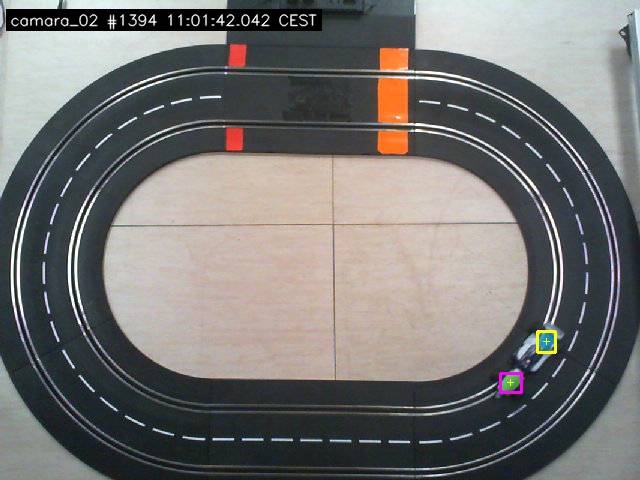
\includegraphics[width=\textwidth]{imaxes/IMPLEMENTACION/derrape_seq_d_recuperado.png}
%        \caption{Seguimiento readquirido}
%        \label{fig:secuencia-derrape-d}
%    \end{subfigure}
%    \caption{Ejemplo de proceso de derrape en el circuito en forma de ovalo}
%    \label{fig:secuencia-derrape}
%\end{figure}
%
%\subsection{Castigo de zonas y ciclo de aprendizaje}
%\label{subsec:algoritmo-aprendizaje}
%
%Las zonas y las dos políticas que actúan sobre ellas se definieron en la sección~\ref{subsec:zonas-politicas}. Cada instancia mantiene la partición de su cadena de celdas en zonas, aplica la política de castigo al cerrarse un derrape y la de mejora al completarse una vuelta.
%
%Cada derrape cerrado desencadena el castigo. El intervalo de celdas del derrape se extiende hacia atrás una distancia fija en píxeles, que es el tramo de anticipación que exige la arquitectura, y el resultado se convierte en una zona de derrape. Su PWM se fija en el mínimo de los de las zonas que cubría el intervalo, menos una reducción fija (de dos unidades), con el parámetro \texttt{minimum\_speed} (sección~\ref{subsec:params-yaml}) como suelo.
%
%Si el derrape cae dentro o junto a una zona de derrape ya existente, ambas se fusionan. El intervalo resultante es la unión de los dos y el PWM, el mínimo de ambos menos la reducción. En ese caso el retroceso añadido es menor que el de una zona nueva, porque la zona existente ya aplicó el suyo al crearse. Si cada reincidencia retrocediera de nuevo la distancia completa, las zonas protegidas acabarían cubriendo el circuito entero y el perfil no volvería a subir en ningún tramo. Las celdas gigantes alcanzadas por un derrape o por su retroceso se castigan como una unidad, ya que dentro del hueco no hay precisión que permita distinguir una parte de otra.
%
%La política de mejora se dispara con el paso por meta. El controlador comprueba si durante la vuelta hubo algún derrape en alguna de las cámaras y comunica el resultado a todas las instancias. Cada zona sin derrape incrementa su PWM en una unidad, con \texttt{maximum\_speed} como techo. Quedan fuera las zonas que registraron un derrape en las últimas vueltas, que permanecen protegidas durante un número configurable de vueltas antes de poder volver a subir.
%
%Las figuras~\ref{fig:derrape-trazas} y~\ref{fig:derrape-dist} recorren el ciclo completo sobre tres vueltas consecutivas de una sesión, con las gráficas de la herramienta de análisis (sección~\ref{subsec:visualizacion-analisis}). En la vuelta~21 la trasera va pegada a la trayectoria base y la distancia nunca se acerca al umbral, de modo que el PWM se mantiene igual en todo el recorrido y solamente hay una zona. En la~22 la trasera se abre en la curva y la distancia lo supera durante diez fotogramas, lo que cierra un derrape y castiga la zona. En la~23 el perfil ya trae el PWM rebajado en ese tramo.
%
%\begin{figure}[tbp]
%    \centering
%    \begin{subfigure}[b]{0.48\textwidth}
%        \centering
%        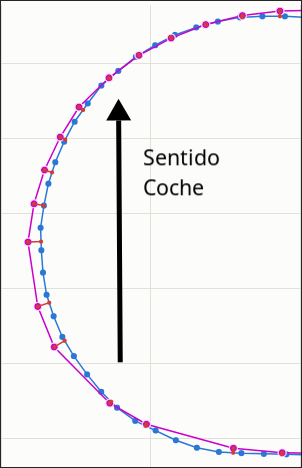
\includegraphics[width=\textwidth]{imaxes/IMPLEMENTACION/derrape_traza_v21.png}
%        \caption{Vuelta 21, limpia}
%        \label{fig:derrape-trazas-a}
%    \end{subfigure}
%    \hfill
%    \begin{subfigure}[b]{0.48\textwidth}
%        \centering
%        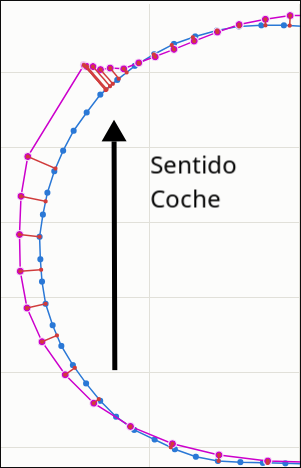
\includegraphics[width=\textwidth]{imaxes/IMPLEMENTACION/derrape_traza_v22.png}
%        \caption{Vuelta 22, con derrape}
%        \label{fig:derrape-trazas-b}
%    \end{subfigure}
%
%    \vspace{0.7em}
%    \begin{subfigure}[b]{0.48\textwidth}
%        \centering
%        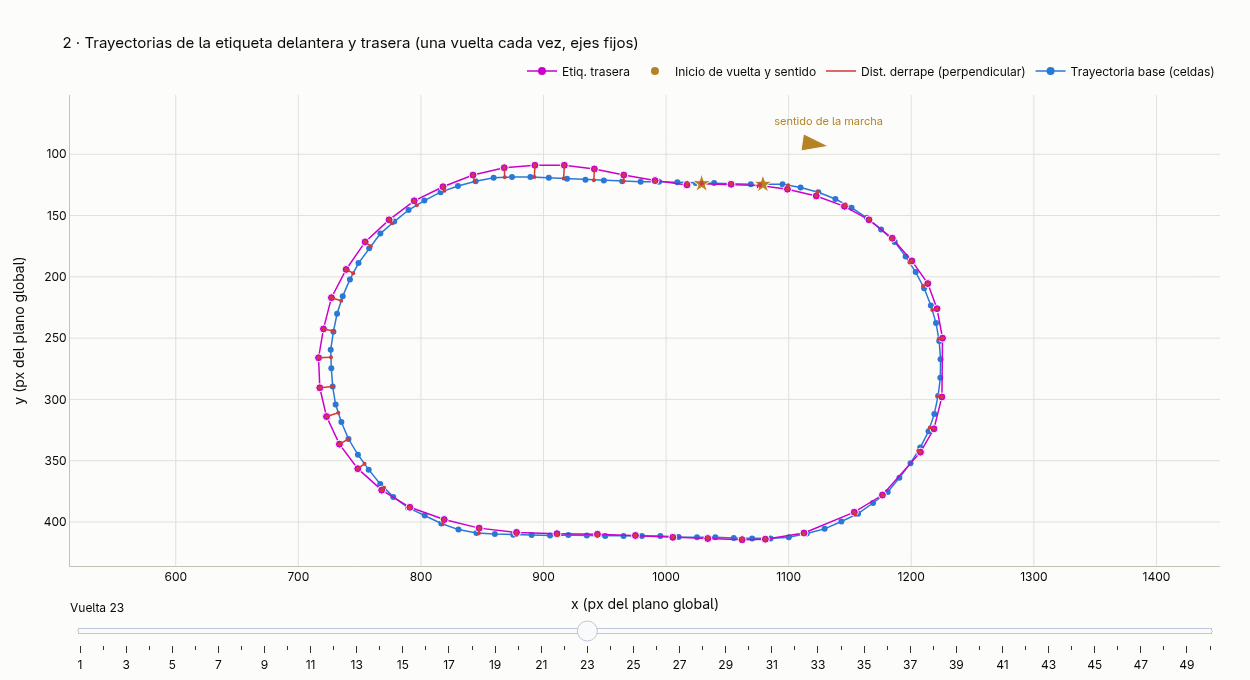
\includegraphics[width=\textwidth]{imaxes/IMPLEMENTACION/derrape_traza_v23.png}
%        \caption{Vuelta 23, ya castigada}
%        \label{fig:derrape-trazas-c}
%    \end{subfigure}
%    \caption{Recorrido de la pegatina trasera (magenta) frente a la trayectoria base (azul) en tres vueltas consecutivas. Los segmentos rojos son la distancia perpendicular que mide el algoritmo}
%    \label{fig:derrape-trazas}
%\end{figure}
%
%\begin{figure}[p]
%    \centering
%    \begin{subfigure}[b]{0.85\textwidth}
%        \centering
%        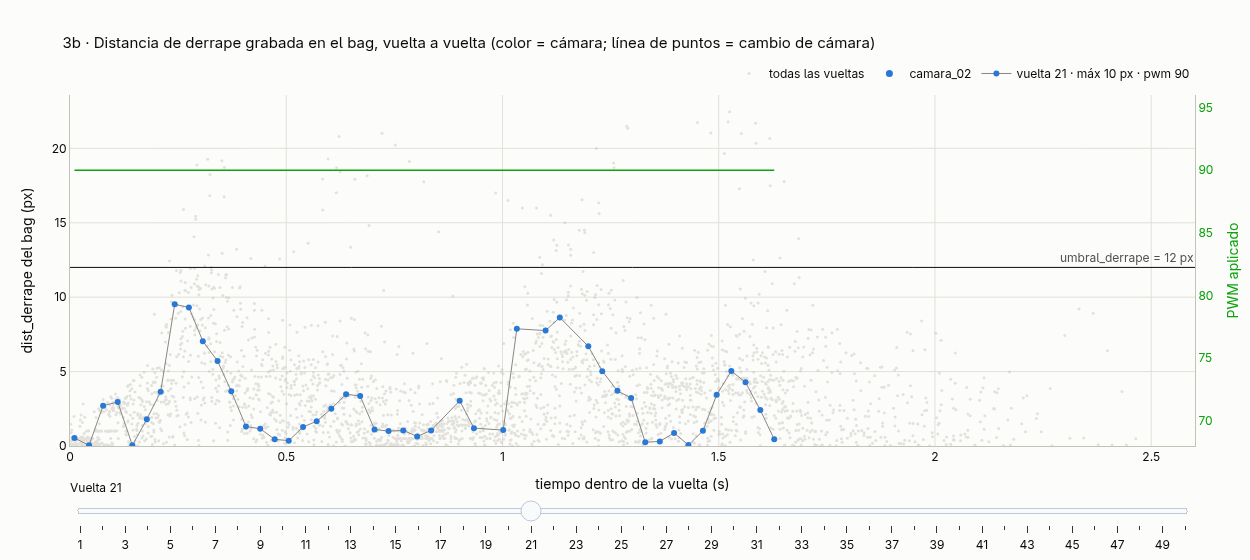
\includegraphics[width=\textwidth]{imaxes/IMPLEMENTACION/derrape_dist_v21.png}
%        \caption{Vuelta 21}
%        \label{fig:derrape-dist-a}
%    \end{subfigure}
%
%    \vspace{0.5em}
%    \begin{subfigure}[b]{0.85\textwidth}
%        \centering
%        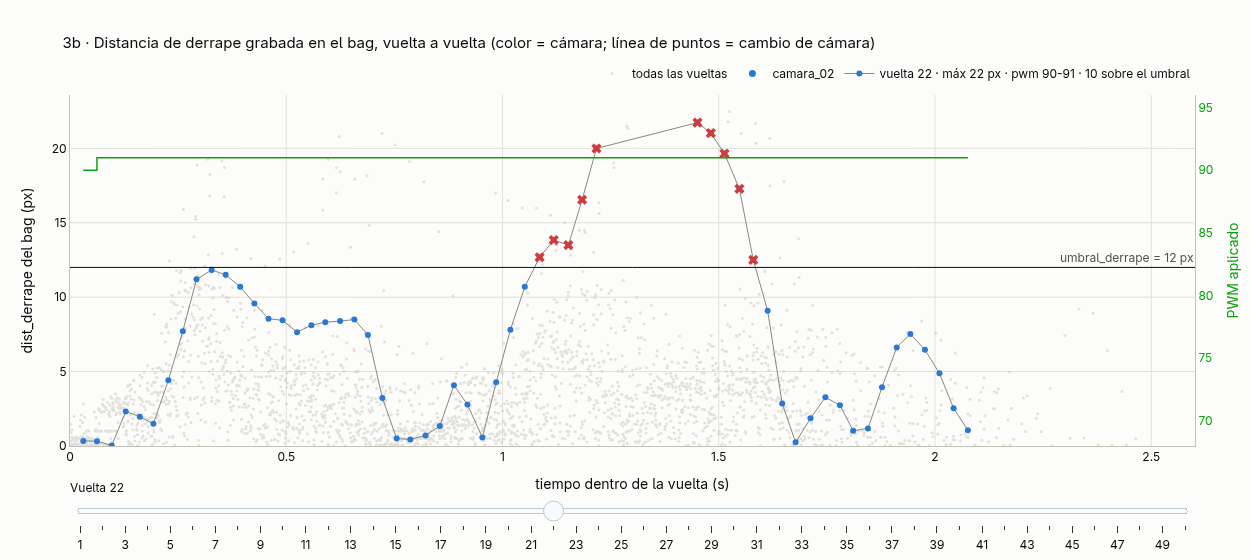
\includegraphics[width=\textwidth]{imaxes/IMPLEMENTACION/derrape_dist_v22.png}
%        \caption{Vuelta 22}
%        \label{fig:derrape-dist-b}
%    \end{subfigure}
%
%    \vspace{0.5em}
%    \begin{subfigure}[b]{0.85\textwidth}
%        \centering
%        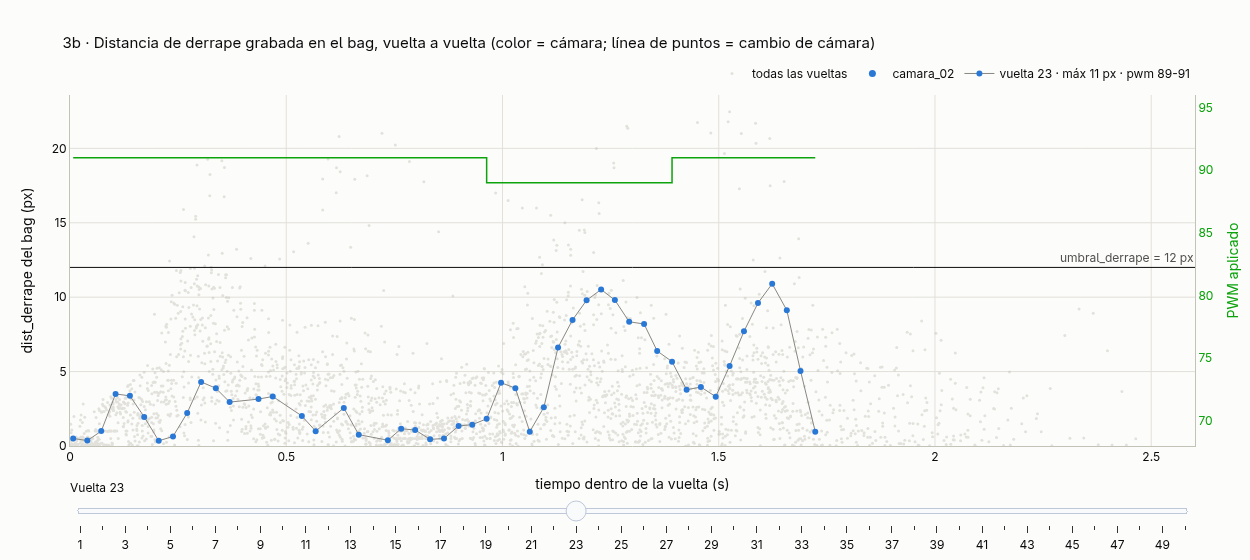
\includegraphics[width=\textwidth]{imaxes/IMPLEMENTACION/derrape_dist_v23.png}
%        \caption{Vuelta 23}
%        \label{fig:derrape-dist-c}
%    \end{subfigure}
%    \caption{Distancia de la pegatina trasera a lo largo de cada vuelta (eje izquierdo) frente al PWM aplicado (línea verde, eje derecho). Las aspas rojas marcan las muestras que superan el umbral y abren el derrape. El escalón verde de la vuelta~23 es la zona creada por el castigo de la anterior.}
%    \label{fig:derrape-dist}
%\end{figure}
%
%\subsection{Coordinación entre cámaras}
%\label{subsec:algoritmo-coordinacion}
%
%Cada instancia conoce solo su porción del circuito (sección~\ref{subsec:algoritmo-instancias}), de modo que hay tres situaciones que ninguna puede resolver por sí sola y que asume el controlador.
%
%La primera es la transición del coche entre cámaras. Cuando dos campos de visión se solapan, ambas publican posiciones intercaladas del mismo coche, así que la cámara activa se mantiene mientras siga entregando fotogramas válidos y solo se cambia a otra cuando deja de hacerlo durante un breve intervalo y esa otra sí está entregando. En cada cambio el controlador notifica la pérdida de visión a la cámara saliente. Como el coche recorre siempre el circuito en el mismo sentido, tras una vuelta completa ese registro contiene el orden secuencial de las cámaras, aprendido en carrera y sin configuración manual.
%
%La segunda es el derrape repartido entre dos cámaras. Al recibir la notificación de pérdida de visión, la instancia saliente cierra el derrape que tuviera abierto y la entrante recibe la orden de abrir uno nuevo, en caso de que el derrape siguiera activo. La zona de derrape se extiende así entre cámaras y el derrape se detecta aunque el corte entre cámaras caiga en mitad de una curva.
%
%La tercera es la propagación de reducciones. Ocurre cuando un derrape se produce cerca del inicio de la porción visible de una cámara, algo habitual si una curva queda repartida entre dos cámaras. El retroceso del castigo se sale por el inicio antes de agotarse y los píxeles restantes corresponden a un tramo de otra cámara. La instancia anota ese sobrante como reducción pendiente; el controlador la recoge tras procesar cada posición y, según el orden aprendido, ordena a la cámara precedente que la aplique al final de su trayectoria, creando o ampliando allí la zona de derrape. Esa reducción externa no incrementa el contador de derrapes de quien la recibe, porque ese derrape ya lo contabilizó la cámara que lo observó, pero la zona queda protegida igual. Si tampoco llegara la trayectoria de la camara anterior, el sobrante volvería a quedar pendiente y se propagaría en poco hacia atrás hasta terminarse.
%
%\section{Nodo de actuación}
%\label{sec:sistema-actuacion}
%
%El nodo de actuación envía hacia el Arduino los valores de PWM calculados por los controladores. Está formado por dos componentes, en primer lugar el nodo puente de ROS~2, que centraliza la recepción de las consignas de todos los controladores, y en segundo lugar el subsistema hardware, compuesto por la placa Arduino y el módulo controlador de motores (L293D).
%
%\subsection{Tratamiento de las consignas recibidas}
%\label{subsec:actuacion-topics}
%
%El nodo puente es un nodo puramente consumidor, no publica nada, se limita a suscribirse a los \emph{topics} en los que cada controlador anuncia el PWM de su carril. Las suscripciones se generan dinámicamente, una por cada coche declarado en la lista de configuración, \ref{subsec:params-yaml}.
%
%De cada mensaje extrae el identificador del carril y su valor de PWM, y le aplica dos comprobaciones antes de mandarlo al puerto serie. La primera es un filtro de repetición, el nodo guarda el último valor enviado a cada carril y descarta el mensaje si coincide con él. Como los controladores publican una consigna por cada posición recibida y el PWM se mantiene estable durante tramos enteros del circuito, este filtro reduce drásticamente el tráfico sobre el puerto. La segunda es una validación del rango admitido por el hardware, entre 0 y 255, como última barrera frente a consignas mal formadas.
%
%El nodo se suscribe también al \emph{topic} de calibración de cada coche que este configurado para control automatico. Durante esa fase es él quien aplica al carril un valor de potencia que permite tener una velocidad de calibración constante, porque los controladores todavía no publican consigna alguna. En cuanto un coche cierra su vuelta se pasa a aplicar el valor que publica el controlador. Los carriles de los coches marcados como manuales no se tocan en ningún momento.
%
%\subsection{Comunicación con el Arduino}
%\label{subsec:actuacion-interfaz}
%
%La comunicación con la placa se encapsula, como en el trabajo de Adrián Rego~\cite{tfgadrian}, en una clase independiente que forma parte del nodo y que abstrae, la complejidad de la comunicación con el puerto serie, en operaciones de alto nivel: fijar la velocidad de un carril, la de ambos o detenerlos. Al inicializarse enumera los puertos disponibles y, si el configurado no está, toma el primer dispositivo compatible que encuentre; después espera a que la placa termine de reiniciarse, vacía el búfer de entrada y detiene ambos carriles, de modo que el sistema arranca siempre desde un estado seguro.
%
%El protocolo es textual y mínimo. Cada orden es una línea de la forma \texttt{r<carril>:<valor>}, por ejemplo \texttt{r1:120}, donde el primer campo identifica el carril y el segundo el PWM a aplicar. El envío es bloqueante, tras escribir la orden la interfaz espera la confirmación de la placa (\texttt{OK}) y solo entonces da la operación por completada; si no llega dentro del tiempo límite, el envío se considera fallido. Aquí ese carácter bloqueante es lo que serializa el acceso.
%
%\subsection{Subsistema hardware}
%\label{subsec:actuacion-hardware}
%
%El subsistema hardware traduce las órdenes recibidas por el puerto serie en la tensión que se aplica sobre los raíles. El montaje es el del trabajo de Adrián Rego~\cite{tfgadrian} y se reutiliza sin cambios. La placa se conecta al ordenador por USB, que es a la vez el canal serie y la alimentación de los motores, y del módulo controlador parten hacia la pista una masa común y dos salidas de potencia, una por carril. Los componentes se describen en la sección~\ref{sec:tecnoloxias-hardware}.
%
%Sobre la placa corre un firmware sencillo, cargado con el IDE de Arduino, que configura los pines de salida PWM, lee el puerto serie a la espera de órdenes y, por cada línea recibida, aplica la señal sobre el pin del carril indicado y responde con la confirmación que la interfaz espera. El ciclo de trabajo del pin es proporcional al valor recibido: 0 corresponde a un ciclo nulo, con el carril detenido, y 255 al ciclo completo; de ahí sale el rango que valida el nodo puente.
%
%Lo que aporta este trabajo no es el montaje, sino su encaje en la arquitectura distribuida. En el trabajo previo la interfaz vivía dentro de una aplicación de escritorio que era también quien procesaba las imágenes y decidía las velocidades; aquí queda detrás del nodo puente el cual permite una comunicación y controla el acceso.
%
%\section{Sistema de visualización y análisis}
%\label{sec:sistema-visualizacion}
%
%El sistema de visualización se compone de dos herramientas independientes que solo se comunican a través de los ficheros que una genera y la otra consume. La de grabación se despliega junto al resto del sistema mientras la sesión está en marcha y almacena todos los mensajes que circulan por la red, en cambio, la de análisis coge la informacion en diferido. Se ejecuta si el usuario quiere al terminar y recibe como entrada el bag generado y los \emph{logs} de los algoritmos a partir de los cuales construye un \emph{dashboard} web que permite estudiar la carrera vuelta a vuelta (figura~\ref{fig:flujo-visualizacion}).
%
%\begin{figure}[H]
%    \centering
%    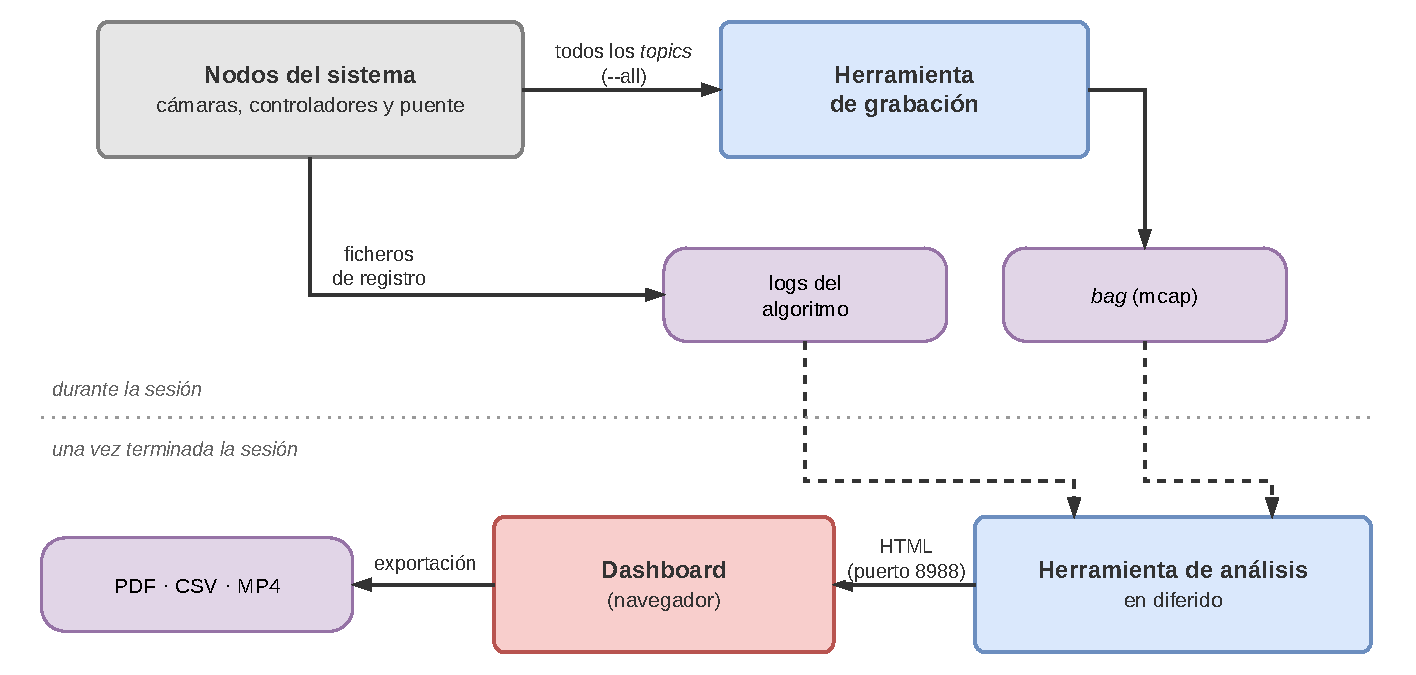
\includegraphics[width=\textwidth]{imaxes/IMPLEMENTACION/flujo_analisis_sistema.pdf}
%    \caption{Esquema que permite ver como es el flujo que se realiza dentro del sistema de analisis}
%    \label{fig:flujo-visualizacion}
%\end{figure}
%
%\subsection{Herramienta de grabación}
%\label{subsec:visualizacion-grabacion}
%
%La herramienta de grabación tiene como cometido capturar sin pérdidas todo el tráfico de la red durante una sesión y dejarlo en disco, sin procesar ni interpretar nada. Se construye sobre \emph{rosbag2} (sección~\ref{sec:ros2-rosbag}), empaquetada en un contenedor junto con las definiciones de los mensajes propios del proyecto, que hay que compilar dentro para que pueda interpretarlos.
%
%La herramienta soporta un descubrimiento dinamico lo que permite grabar sin conocer de antemano qué nodos van a estar presentes. Una primera versión trabajaba con una lista explícita de \emph{topics}, construida a partir del número de cámaras y coches configurados, y resultó una fuente constante de errores porque por cada \emph{topic} nuevo o renombrado había que acordarse de reflejarlo en ella. La versión definitiva graba la totalidad de los \emph{topics} y sondea periódicamente en busca de otros, suscribiéndose a los que van apareciendo, de modo que no impone ningún orden de arranque. La calidad de servicio se resuelve igual, en lugar de mantener un fichero que reprodujera las políticas del sistema, la herramienta adapta el perfil de cada suscripción al que ofrecen los publicadores que encuentra.
%
%Se escogio el formato \emph{mcap} porque lleva embebida la definición de cada mensaje lo que permite poder seguir analizando todos los bags aunque no dispongamos ya de la definion de los mensajes, esto es debido a que los mensajes del sistema fueron evolucionando conforme avanzaba el proyecto.
%
%\subsection{Herramienta de análisis en diferido}
%\label{subsec:visualizacion-analisis}
%
%La herramienta de análisis convierte los datos crudos de una sesión en un conjunto de gráficas. Combina dos fuentes: la grabación(\emph{bags}), de la que obtiene todo lo que se publicó en la red, y los ficheros de \emph{logs} que escribe el algoritmo, de los que obtiene su estado interno. La primera describe qué hizo el coche y los segundos explican por qué el sistema decidió lo que decidió, de modo que solo cruzando ambas se puede relacionar un comportamiento con la decisión que lo provocó.
%
%El resultado es un \emph{dashboard}, una página web autocontenida con gráficas interactivas que permiten desplazarse, ampliar una zona y consultar el valor de cada punto, organizada en las secciones numeradas que recoge el cuadro~\ref{tab:secciones-dashboard}. Como cada cámara trabaja en sus propias coordenadas de imagen, todas las gráficas espaciales se dibujan sobre un plano global común, aplicando a cada cámara una traslación fija. Desde el propio \emph{dashboard} pueden exportarse las gráficas en PDF, los datos en CSV y descargar un vídeo que combina las imágenes de todas las cámaras.
%
%También el análisis se ejecuta en un contenedor, que a diferencia del resto no forma parte del sistema desplegado. Se levanta bajo demanda indicándole qué sesión analizar, genera el \emph{dashboard}, lo sirve en un puerto accesible desde la máquina anfitriona y termina al pararlo. Necesita contenedor por la misma razón que la grabación, leer ficheros mcap exige tener disponibles las bibliotecas de ROS~2 y las definiciones de los mensajes.
%
%\begin{table}[htbp]
%\centering
%\resizebox{\textwidth}{!}{
%\begin{tabular}{|c|l|}
%\hline
%\rowcolor{ArqAzulClaro}
%\textbf{Sección} & \textbf{Contenido} \\
%\hline
%0 & Resumen de la sesión \\
%\hline
%1 & Valor del derrape en cada punto del recorrido (3D) \\
%\hline
%2 & Trayectorias de las etiquetas delantera y trasera \\
%\hline
%3 & Distancia de derrape de la etiqueta trasera \\
%\hline
%4 & Mapa del circuito con el PWM de cada celda \\
%\hline
%5 & Tiempos por vuelta \\
%\hline
%6 & Evolución de las zonas, perfil de PWM y resumen por vuelta \\
%\hline
%7 & Visor de las imágenes grabadas y generación de vídeo \\
%\hline
%8 & Descarga de los datos en formato CSV \\
%\hline
%\end{tabular}
%}
%\caption{Secciones del \emph{dashboard} generado por la herramienta de análisis.}
%\label{tab:secciones-dashboard}
%\end{table}
%




\chapter{Implementación del diseño}
\label{chap:implementacion}

\lettrine{E}{N} este capítulo se describe cómo se llevó a código la arquitectura del capítulo~\ref{chap:arquitectura}. No se repite qué hace cada nodo, sino cómo se resolvieron los problemas que aparecieron al programarlo: cómo se despliega el sistema, cómo reparte cada proceso su trabajo, qué se hace con cada fotograma, cómo se decide la potencia de cada carril y qué desviaciones aparecieron respecto al diseño inicial.

\section{Despliegue y configuración}
\label{sec:configuracion_despliegue}

El número de cámaras y de coches, y su reparto entre máquinas, no está fijado en el código: se decide al desplegar el sistema (sección~\ref{sec:despliegue_sistema}). Esa flexibilidad descansa sobre tres piezas: un fichero de parámetros común, un fichero de lanzamiento por componente y un contenedor que lo ejecuta.

\subsection{Parámetros y lanzamiento}
\label{subsec:params-yaml}
\label{subsec:launch-files}

Toda la configuración se centraliza en un único \texttt{params.yaml} que comparten todos los nodos y que puede consultarse íntegro en el anexo~\ref{lst:params-yaml}. Cada nodo declara solo los parámetros que le interesan y descarta el resto, y buena parte de ellos admite modificación en caliente, de modo que ajustar un umbral no obliga a relanzar el sistema.

De todo el fichero, solo dos entradas fijan la escala del despliegue. La lista \texttt{coches} enumera los vehículos presentes y de ella se deriva lo demás: cuántos detectores crea cada cámara, cuántos controladores se levantan y a qué \emph{topics} se suscribe el puente. El bloque \texttt{cars} describe cada coche por su nombre —los colores de sus dos pegatinas, que son lo que permite seguir a varios a la vez sin confundirlos, el carril que ocupa y un indicador \texttt{modo\_manual} que decide si lo conduce el sistema o una persona—. El resto agrupa por componente la resolución y los umbrales de visión, los límites del perfil de velocidad y los datos del puerto serie.

Sobre ese fichero se apoyan los ficheros de lanzamiento, uno por componente y todos con el mismo patrón: leen los parámetros comunes, crean los nodos y les asignan un espacio de nombres. El del nodo de captura (anexo~\ref{lst:camera-launch}) es el más simple, porque solo recibe el identificador del nodo y el dispositivo de vídeo y los inyecta como parámetros. Los otros dos deciden en el propio lanzamiento cuántos nodos crear: recorren la lista \texttt{coches} y levantan un controlador por cada uno, filtrando por \texttt{modo\_manual}. El principal (anexo~\ref{lst:brain-launch}) se queda con los coches autónomos y añade el nodo puente; el de carrera manual (anexo~\ref{lst:manual-launch}) se queda con los conducidos por una persona y no lo arranca, porque en ese caso ningún controlador publica consigna. Como ambos filtran la misma lista por criterios opuestos, una carrera mixta se consigue levantando los dos a la vez.\footnote{Cada controlador recibe un nombre de nodo derivado del coche y del modo, porque los ficheros de \emph{log} del algoritmo se nombran a partir del nodo y dos homónimos se pisarían.}

Todos los nodos se declaran con reinicio automático y un retardo entre intentos. Si uno cae durante una sesión, el sistema lo relanza y se reincorpora por sí solo gracias al descubrimiento del \emph{middleware}, comportamiento que se valida en la prueba de tolerancia a fallos de la sección~\ref{subsec:prueba-tolerancia}.

\subsection{Despliegue en contenedores}
\label{subsec:despliegue-docker}

Cada componente se despliega en un contenedor Docker construido sobre una imagen común, derivada de la oficial de ROS~2 y ampliada con las bibliotecas de visión y de comunicación serie. Una máquina solo necesita, por tanto, Docker y conectividad de red: no hace falta instalar ROS~2 ni ninguna dependencia en el anfitrión, que es justo lo que exigía la sección~\ref{sec:despliegue_sistema}.

Los ficheros \emph{compose} comparten la misma base, que puede verse en el del nodo de captura (anexo~\ref{lst:compose-camera}). Los contenedores usan la pila de red y la memoria compartida del anfitrión y fijan el mismo identificador de dominio (sección~\ref{sec:dds-qos}): con la red del anfitrión los nodos se descubren entre máquinas, y la memoria compartida permite que, cuando dos coinciden en la misma máquina, la capa de comunicación lo detecte y los comunique directamente sin pasar por la red. Todos montan además el paquete desde el anfitrión, para conservar los ficheros que escriben los nodos cuando el contenedor se para, y fijan la zona horaria, ya que la imagen base trabaja en UTC. Las diferencias entre ellos son mínimas: el de captura recibe por variables de entorno su identificador y su dispositivo de vídeo, el del cerebro (anexo~\ref{lst:compose-brain}) es el único que mapea el puerto serie del Arduino y el de modo manual (anexo~\ref{lst:compose-manual}) prescinde de ese mapeo, de forma que arranca aunque la placa ni siquiera esté conectada.

\section{Modelo de ejecución concurrente}
\label{concurrencia}

La concurrencia interna que exige la arquitectura (sección~\ref{sec:concurrencia}) se resuelve con los \emph{executors} y los grupos de \emph{callbacks} de ROS~2 (sección~\ref{sec:ros2-executors}). Todos los nodos corren sobre un \emph{MultiThreadedExecutor} y reparten sus tareas entre varios \emph{MutuallyExclusiveCallbackGroup} siguiendo un criterio doble: los \emph{callbacks} que tocan el mismo estado interno van al mismo grupo, y las tareas independientes van a grupos distintos. Lo primero evita tener que proteger el estado con cerrojos y lo segundo evita que una tarea espere por otra. La figura~\ref{fig:concurrencia-nodos} recoge el reparto resultante en los tres tipos de nodo.

\begin{figure}[tbp]
    \centering
    \begin{subfigure}[b]{0.9\textwidth}
        \centering
        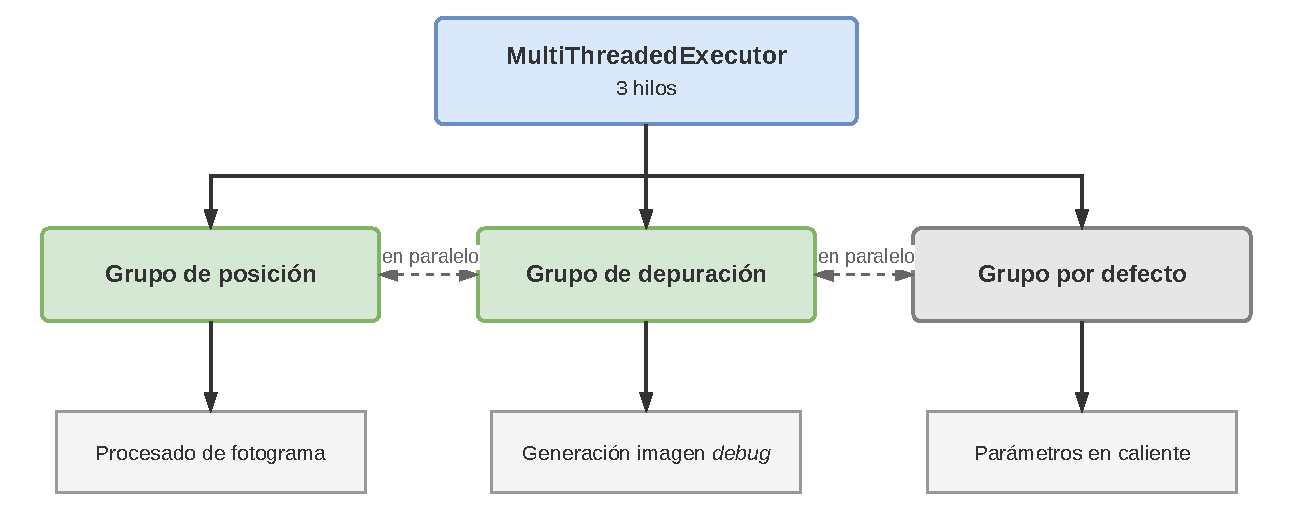
\includegraphics[width=\textwidth]{imaxes/IMPLEMENTACION/multithread_nodo_camara.pdf}
        \caption{Nodo de captura}
        \label{fig:executor-multihilo}
    \end{subfigure}

    \vspace{0.6em}
    \begin{subfigure}[b]{0.9\textwidth}
        \centering
        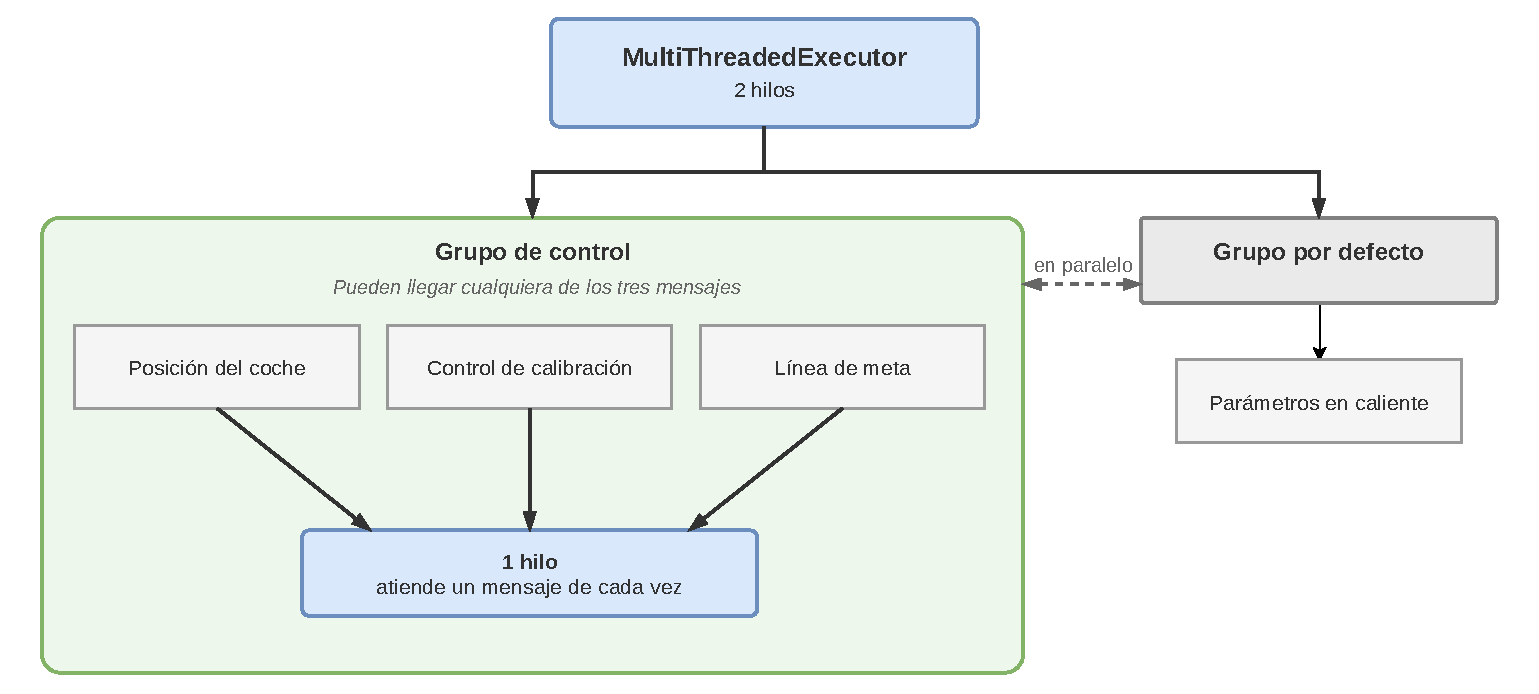
\includegraphics[width=\textwidth]{imaxes/IMPLEMENTACION/multithread_nodo_controlador.pdf}
        \caption{Nodo de control de carril}
        \label{fig:concurrencia-controlador}
    \end{subfigure}

    \vspace{0.6em}
    \begin{subfigure}[b]{0.8\textwidth}
        \centering
        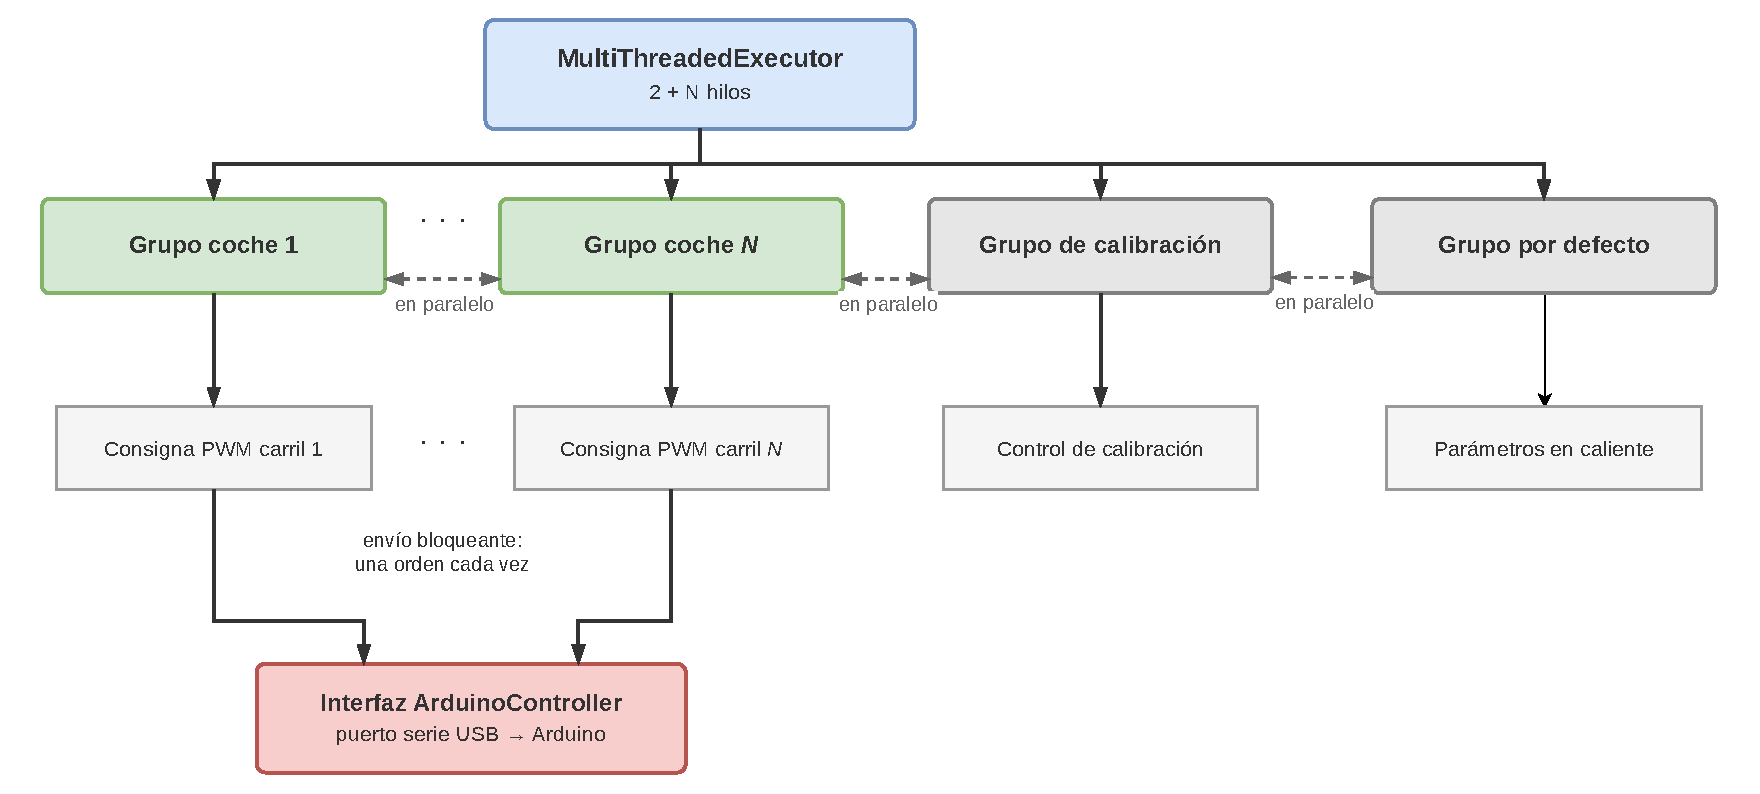
\includegraphics[width=\textwidth]{imaxes/IMPLEMENTACION/multithread_nodo_puente.pdf}
        \caption{Nodo puente}
        \label{fig:concurrencia-puente}
    \end{subfigure}
    \caption{Reparto de los \emph{callbacks} en grupos dentro de cada tipo de nodo. En los tres casos se conserva el grupo por defecto de ROS~2, atendido por un hilo propio, que es el que mantiene disponible la reconfiguración en caliente.}
    \label{fig:concurrencia-nodos}
\end{figure}

El nodo de captura es el más exigente, porque atiende dos tareas de coste muy distinto: obtener las posiciones de los coches y generar las imágenes de depuración. Cada una tiene su grupo, de modo que la segunda nunca retrasa a la primera. Dentro del procesamiento hay además un segundo nivel de concurrencia, porque buscar varios coches en un mismo fotograma multiplica el trabajo por vehículo. Se resolvió con un patrón productor-consumidor (figura~\ref{fig:modelo-hilos-camara}): el productor recoge los fotogramas que entrega la cámara cada \qty{33}{\milli\second} y un \emph{timer} de ROS~2 toma el último y lanza su procesamiento sobre un \emph{ThreadPool} con un trabajador por coche. Como la búsqueda de cada coche es independiente de las demás, todas se ejecutan sobre el mismo fotograma a la vez y el consumidor espera a que terminen antes de darlo por procesado. Un \emph{flag} impide que un disparo se solape con un procesamiento en curso: si el análisis se prolonga, los disparos intermedios se descartan en lugar de encolarse, con lo que el nodo degrada su cadencia pero nunca acumula retraso.

\begin{figure}[tbp]
    \centering
    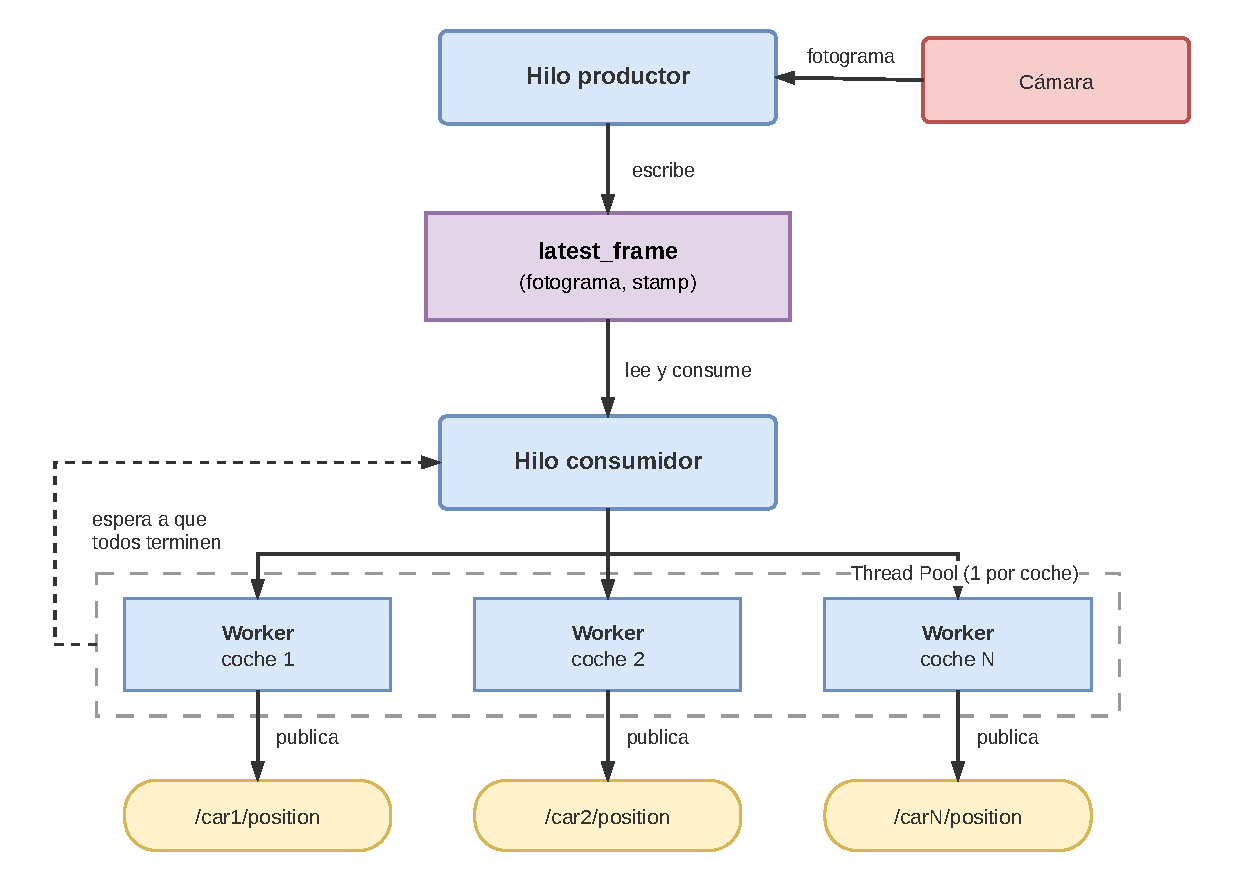
\includegraphics[width=0.75\textwidth]{imaxes/IMPLEMENTACION/productor_consumidor_nodo_camara.pdf}
    \caption{Modelo productor-consumidor con el que el nodo de cámara busca todos los coches sobre un mismo fotograma.}
    \label{fig:modelo-hilos-camara}
\end{figure}

Los otros dos nodos solo necesitan concurrencia a nivel de nodo. El controlador recibe la posición del coche, la orden de cambio de modo y la línea de meta, y como los tres modifican el mismo estado van a un único grupo, con lo que el estado del algoritmo queda siempre en manos de un solo hilo. El puente, en cambio, crea un grupo por controlador desplegado, ya que cada uno publica en su propio \emph{topic} y así el retraso de un carril no impide atender los demás. Esa concurrencia, sin embargo, no llega al envío: hay un único Arduino y un único puerto serie, y la propia interfaz de comunicación serializa el acceso (sección~\ref{subsec:actuacion-interfaz}).

\section{Detección de las pegatinas}
\label{sec:nodo-camara}
\label{subsec:deteccion-etiquetas}

Todo lo que el sistema sabe de un coche sale de localizar sus dos pegatinas en la imagen, y ese procedimiento se hereda del trabajo de Mario López~\cite{tfgmario}. El fotograma se convierte al espacio HSV, que resiste mejor las variaciones de iluminación, y se genera una máscara binaria por pegatina con los píxeles que caen dentro del rango de su color, predefinido para cada uno de los siete colores admitidos. Sobre esa máscara se encadenan una apertura morfológica, que elimina los píxeles aislados, y un cierre, que rellena los huecos de las regiones válidas. De los contornos externos resultantes se toma el mayor, se descarta si no supera un área mínima configurable y se obtienen su rectángulo delimitador y su centroide. La figura~\ref{fig:deteccion-color} recorre estas etapas sobre un fotograma real.

\begin{figure}[tbp]
    \centering
    \begin{subfigure}[b]{0.48\textwidth}
        \centering
        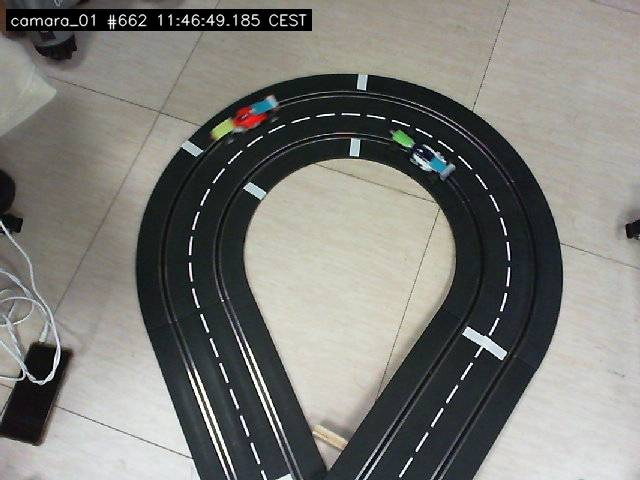
\includegraphics[width=\textwidth]{imaxes/IMPLEMENTACION/det_color_a_original.png}
        \caption{Fotograma capturado}
        \label{fig:deteccion-color-a}
    \end{subfigure}
    \hfill
    \begin{subfigure}[b]{0.48\textwidth}
        \centering
        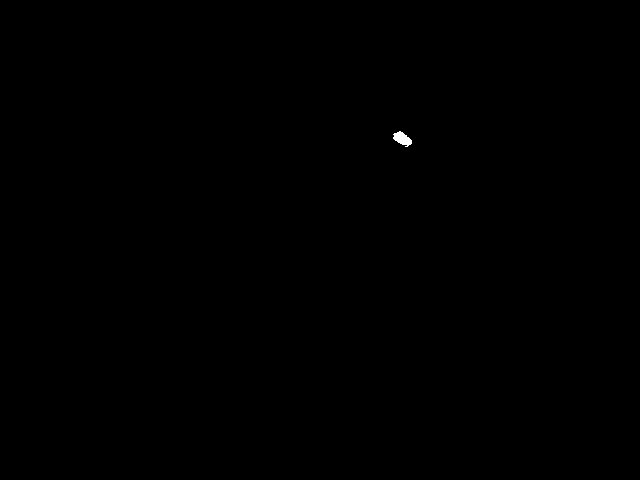
\includegraphics[width=\textwidth]{imaxes/IMPLEMENTACION/det_color_b_mascara.png}
        \caption{Máscara del color de la pegatina delantera}
        \label{fig:deteccion-color-b}
    \end{subfigure}

    \vspace{0.7em}
    \begin{subfigure}[b]{0.34\textwidth}
        \centering
        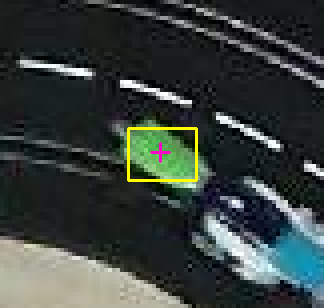
\includegraphics[width=\textwidth]{imaxes/IMPLEMENTACION/det_color_c_resultado.png}
        \caption{Rectángulo y centroide}
        \label{fig:deteccion-color-c}
    \end{subfigure}
    \caption{Etapas de la detección por color de una de las pegatinas del coche.}
    \label{fig:deteccion-color}
\end{figure}

Lo que cambia entre los dos modos de funcionamiento (sección~\ref{sec:modos_funcionamiento}) no es este procedimiento, sino la región del fotograma sobre la que se aplica: la imagen completa durante la calibración y una región reducida durante la carrera.

\section{La vuelta de calibración}
\label{subsec:modos-funcionamiento}
\label{subsec:control-modos}

La calibración produce dos cosas a la vez, una en la cámara y otra en el controlador, a partir del mismo flujo de detecciones de la pegatina delantera. Basta con la delantera porque es la que da una trayectoria limpia~\cite{tfgadrian}: la trasera puede quedar oculta a ratos y la ruta base debe registrarse sin interrupciones. Como consecuencia, las pegatinas delanteras sí deben ser de distinto color entre coches, mientras que dos coches pueden compartir la trasera.

En la cámara, cada detección se acumula hasta que el coche cierra su vuelta; con esos puntos se genera una máscara que restringe la búsqueda de ese coche a una franja alrededor del recorrido conocido (figura~\ref{fig:mascara-trayectoria}). Esa franja deja fuera el carril contrario, con lo que el coche que circula por él deja de ser un falso positivo posible. La calibración termina coche a coche y no para todo el sistema: la cámara se suscribe al \emph{topic} de calibración de cada vehículo configurado y genera su máscara al recibir el aviso correspondiente, de modo que un coche puede estar ya en carrera mientras otro sigue dando su vuelta de reconocimiento.

\begin{figure}[tbp]
    \centering
    \begin{subfigure}[b]{0.32\textwidth}
        \centering
        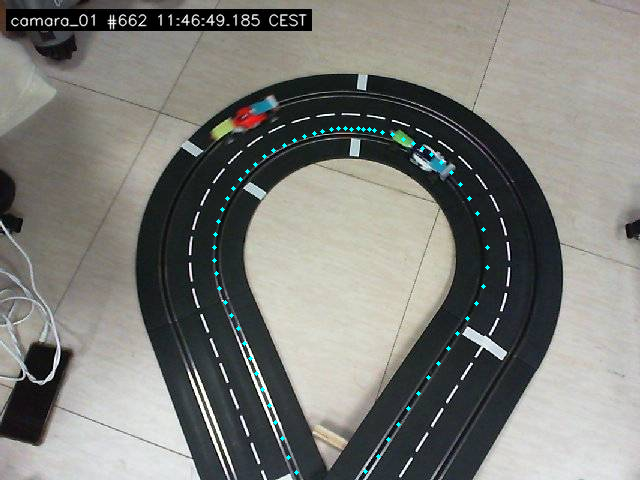
\includegraphics[width=\textwidth]{imaxes/IMPLEMENTACION/mascara_a_puntos.png}
        \caption{Posiciones acumuladas}
        \label{fig:mascara-trayectoria-a}
    \end{subfigure}
    \hfill
    \begin{subfigure}[b]{0.32\textwidth}
        \centering
        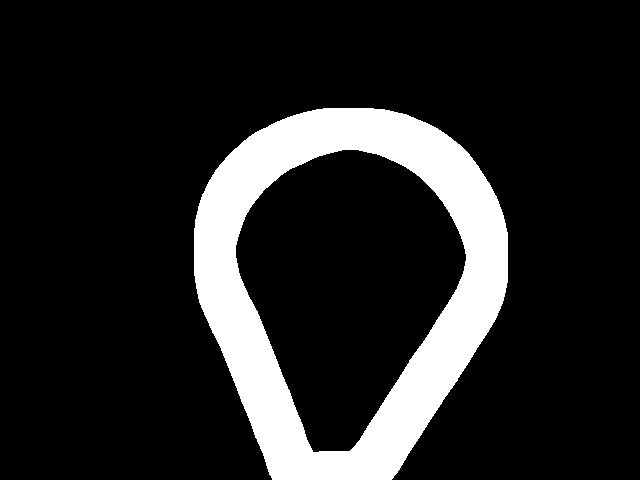
\includegraphics[width=\textwidth]{imaxes/IMPLEMENTACION/mascara_b_mascara.png}
        \caption{Máscara generada}
        \label{fig:mascara-trayectoria-b}
    \end{subfigure}
    \hfill
    \begin{subfigure}[b]{0.32\textwidth}
        \centering
        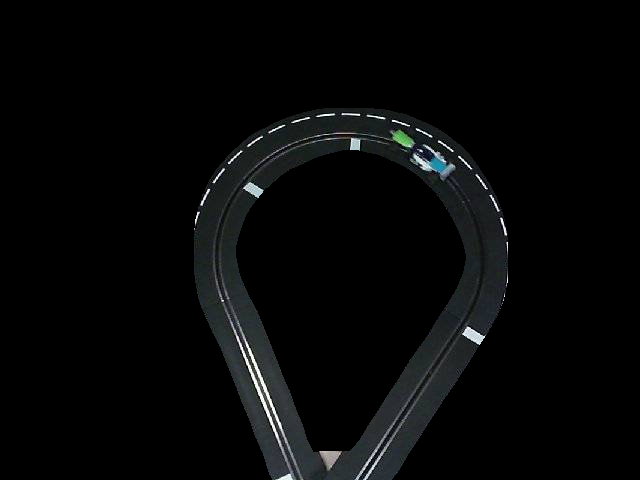
\includegraphics[width=\textwidth]{imaxes/IMPLEMENTACION/mascara_c_filtrado.png}
        \caption{Fotograma filtrado}
        \label{fig:mascara-trayectoria-c}
    \end{subfigure}
    \caption{Generación de la máscara de trayectoria de un coche a partir de su vuelta de calibración.}
    \label{fig:mascara-trayectoria}
\end{figure}

En el controlador, las mismas posiciones se acumulan en un diccionario indexado por cámara: cada nodo de captura del que recibe mensajes tiene su propia lista de puntos y en ningún momento se construye una lista única con el circuito completo. Lo que delimita la acumulación es el paso por meta. Los puntos se recogen entre el primer cruce y el segundo, de modo que cada trayectoria base es exactamente una vuelta que empieza en la meta y todo lo anterior —colocar el coche, arrancarlo y las vueltas que dé mientras se levanta el sistema— se descarta. Al cerrarse la vuelta el controlador lo notifica en su \emph{topic} de calibración, filtra cada lista descartando los puntos que queden a menos de un umbral del último aceptado y crea una instancia del algoritmo por cámara, a la que inyecta su trayectoria. Lo aprendido se vuelca en disco en ficheros JSON, que los nodos cargan al arrancar para saltarse la calibración cuando ni las cámaras ni el circuito se han movido.
\label{subsec:cache-calibracion}

Que la calibración se cierre sola es un requisito de la arquitectura, no una comodidad. En los trabajos previos la arrancaba y la daba por concluida una persona desde una interfaz gráfica: había que delimitar el coche con un rectángulo y marcar la meta a mano~\cite{tfgmario}, o seleccionar el vehículo, activar la búsqueda y confirmar los valores obtenidos~\cite{tfgadrian}. Con los nodos repartidos entre varias máquinas y sin una interfaz desde la que supervisarlos, la única forma de delimitar la vuelta es con la información que ya circula por la red, y esa información es el paso por meta que el propio controlador detecta.

\section{Seguimiento en carrera}
\label{subsec:seguimiento-roi}

Cerrada la calibración, la búsqueda deja de recorrer el fotograma entero y se restringe a una región de interés de $150 \times 150$ píxeles centrada en la posición predicha para el coche, obtenida por la extrapolación lineal que introdujo Mario López~\cite{tfgmario}: conocidas las dos últimas posiciones, el centro de la región es la actual más el vector de movimiento del último fotograma. Sobre ella se aplica además la máscara de trayectoria, de modo que solo sobreviven los píxeles que pertenecen a la vez a la región y a las proximidades del carril; la intersección de ambos filtros procede también de los trabajos previos~\cite{tfgmario,tfgadrian}. La figura~\ref{fig:roi-filtrado} muestra el proceso completo, y su último panel es lo único que llega al detector de color. El precio de trabajar sobre un recorte es que las coordenadas obtenidas son relativas a la región y hay que trasladarlas al sistema de referencia de la cámara antes de publicarlas.

\begin{figure}[tbp]
    \centering
    \begin{subfigure}[b]{0.55\textwidth}
        \centering
        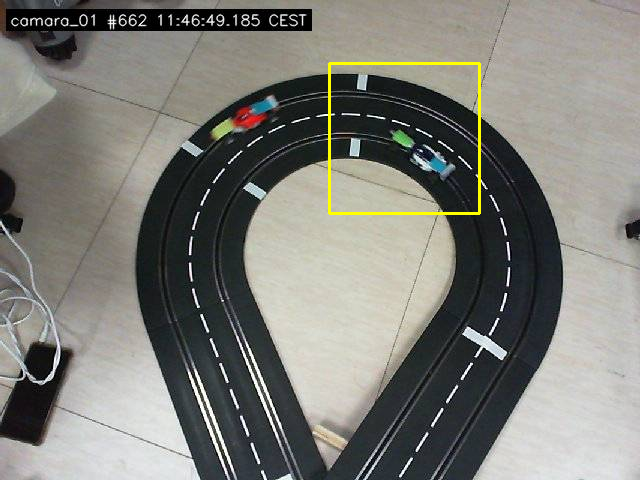
\includegraphics[width=\textwidth]{imaxes/IMPLEMENTACION/roi_a_recuadro.png}
        \caption{Región marcada sobre el fotograma}
        \label{fig:roi-filtrado-a}
    \end{subfigure}
    \hfill
    \begin{subfigure}[b]{0.38\textwidth}
        \centering
        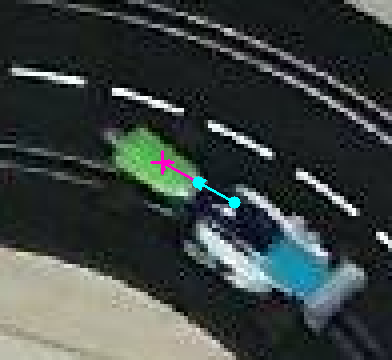
\includegraphics[width=\textwidth]{imaxes/IMPLEMENTACION/roi_b_extrapolacion.png}
        \caption{Extrapolación de la posición}
        \label{fig:roi-filtrado-b}
    \end{subfigure}

    \vspace{0.7em}
    \begin{subfigure}[b]{0.32\textwidth}
        \centering
        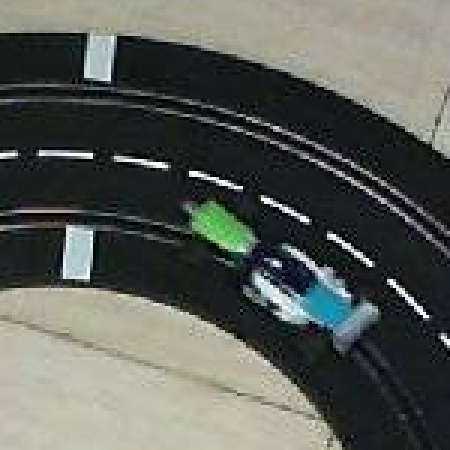
\includegraphics[width=\textwidth]{imaxes/IMPLEMENTACION/roi_c_recorte.png}
        \caption{Recorte de la región}
        \label{fig:roi-filtrado-c}
    \end{subfigure}
    \hspace{0.04\textwidth}
    \begin{subfigure}[b]{0.32\textwidth}
        \centering
        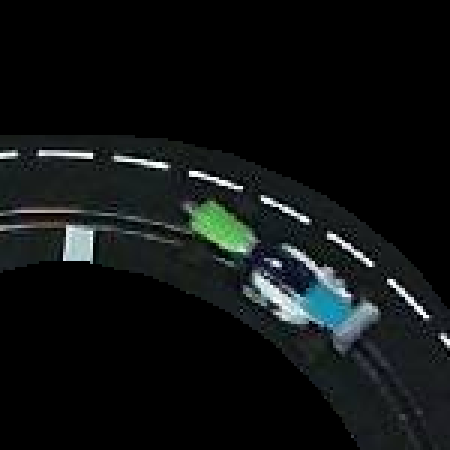
\includegraphics[width=\textwidth]{imaxes/IMPLEMENTACION/roi_d_filtrado.png}
        \caption{Intersección con la máscara}
        \label{fig:roi-filtrado-d}
    \end{subfigure}
    \caption{Acotación de la búsqueda en modo carrera. En el detalle, las dos flechas encadenadas son el desplazamiento medido entre los dos últimos fotogramas y la cruz marca la posición predicha, que en este caso cae a 1,6~píxeles de la real.}
    \label{fig:roi-filtrado}
\end{figure}

Las oclusiones son habituales en un circuito de Scalextric~\cite{tfgmario} y un derrape brusco puede alejar el coche de la posición predicha, así que hay que contar con perder el seguimiento y recuperarlo.
\label{subsec:readquisicion}
La estrategia es ampliar progresivamente la zona de búsqueda: cada fotograma sin detección incrementa el tamaño de la región en 50~píxeles, hasta abarcar como máximo la imagen completa. Los trabajos previos pasaban de golpe a examinar toda la proximidad de la trayectoria; el crecimiento gradual acota el coste de los fotogramas inmediatamente posteriores a la pérdida, que son los más probables. Al perder el seguimiento se descartan además las posiciones anteriores, como ya hacía Mario López~\cite{tfgmario}, para que la extrapolación no combine un punto previo a la pérdida con el primero posterior y sitúe la región lejos del coche; la primera detección tras readquirir vuelve a centrarla sobre la posición encontrada.

Por último, el nodo ofrece un modo de depuración, desactivado por defecto y activable en caliente, que conserva una copia del fotograma procesado y dibuja sobre él los rectángulos de las pegatinas, una cruceta en cada centroide y, en una esquina, el identificador del nodo, el número de fotograma y la hora de captura. Esa imagen se publica como \emph{vista de la cámara} y es la que permite seguir cada cámara en directo y la que graba el sistema de visualización (sección~\ref{sec:sistema-visualizacion}).
\label{subsec:modo-depuracion}

\section{La meta y los tiempos por vuelta}
\label{subsec:deteccion-meta}
\label{sec:control-rail}

La línea de meta se señaliza con una etiqueta alargada de un color reservado que atraviesa la pista y se detecta una sola vez, al arrancar el nodo, porque su posición no cambia durante la carrera. El procedimiento es el de Adrián Rego~\cite{tfgadrian} y arranca igual que la detección de las pegatinas, con la máscara del color en HSV, pero el cierre morfológico se aplica con un \emph{kernel} mucho mayor: los raíles y las ranuras de la pista atraviesan la etiqueta y la fragmentan en trozos que hay que volver a unir en una única región (figura~\ref{fig:deteccion-meta}). Sobre ella se calcula el rectángulo de área mínima que la encierra, que a diferencia del delimitador convencional puede estar rotado y se adapta así a la orientación real de la línea; de sus cuatro vértices se identifican los dos lados cortos comparando las aristas adyacentes, y el segmento que une sus puntos medios define la meta. Cada cámara la busca al arrancar y, si no la ve, no publica nada, de modo que en un despliegue multicámara solo la publica la que la observa y no hay que designar de antemano una cámara de meta.

\begin{figure}[tbp]
    \centering
    \begin{subfigure}[b]{0.32\textwidth}
        \centering
        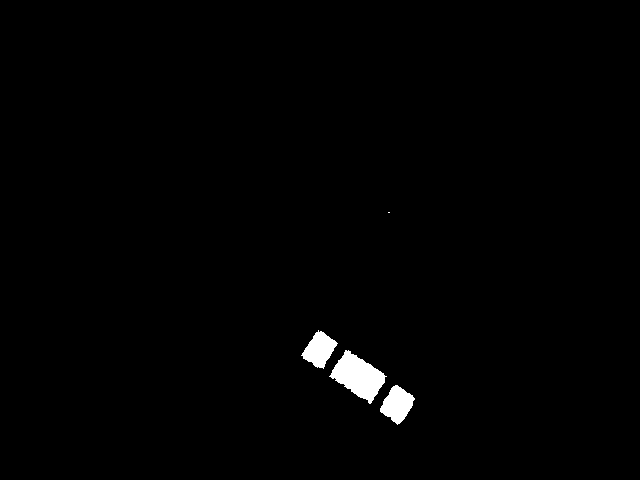
\includegraphics[width=\textwidth]{imaxes/IMPLEMENTACION/meta_a_mascara.png}
        \caption{Máscara del color de la meta}
        \label{fig:deteccion-meta-a}
    \end{subfigure}
    \hfill
    \begin{subfigure}[b]{0.32\textwidth}
        \centering
        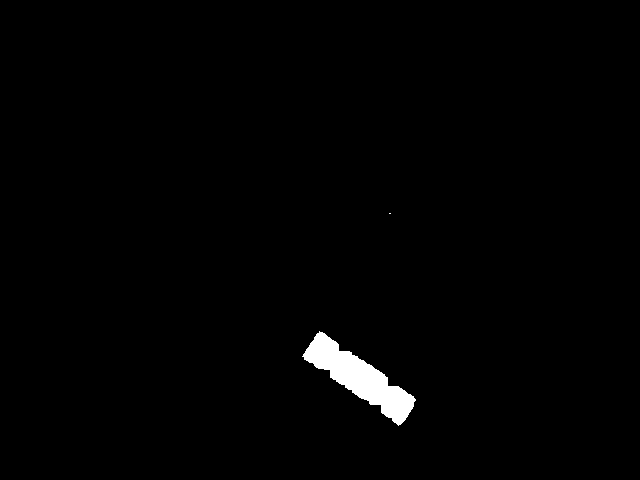
\includegraphics[width=\textwidth]{imaxes/IMPLEMENTACION/meta_b_cierre.png}
        \caption{Tras el cierre morfológico}
        \label{fig:deteccion-meta-b}
    \end{subfigure}
    \hfill
    \begin{subfigure}[b]{0.32\textwidth}
        \centering
        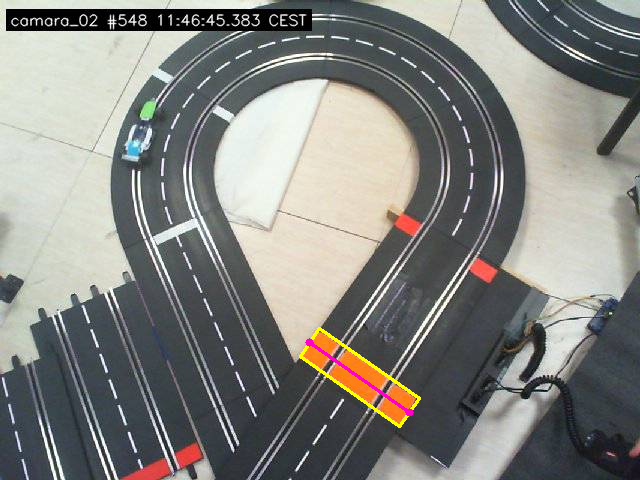
\includegraphics[width=\textwidth]{imaxes/IMPLEMENTACION/meta_c_segmento.png}
        \caption{Rectángulo y segmento}
        \label{fig:deteccion-meta-c}
    \end{subfigure}
    \caption{Detección de la línea de meta en la cámara~2. Los raíles parten la etiqueta en tres trozos que el cierre vuelve a unir.}
    \label{fig:deteccion-meta}
\end{figure}

Con ese segmento, el controlador cuenta las vueltas de su coche y mide su duración, que es lo que cierra el ciclo de aprendizaje del algoritmo (sección~\ref{subsec:algoritmo-aprendizaje}).
\label{subsec:control-meta}
El mecanismo se hereda de Mario López~\cite{tfgmario} y solo se aplica a los mensajes de la cámara que publicó la meta: para cada posición se calcula el producto vectorial entre el vector que recorre el segmento y el que va de uno de sus extremos a la pegatina delantera, y su signo indica de qué lado de la recta está el coche, de modo que un cambio de signo entre dos fotogramas consecutivos significa que lo ha cruzado (figura~\ref{fig:producto-vectorial}). El instante exacto se aproxima interpolando entre los dos fotogramas implicados, con la fracción del intervalo que se obtiene del cociente entre la distancia del anterior y la suma de ambas; sin interpolar, tomar la marca del fotograma que detecta el cruce introduciría un error de hasta un período de captura en cada vuelta. Los instantes interpolados son las marcas de tiempo que la cámara pone al capturar, no el momento en que llega el mensaje (sección~\ref{subsec:qos}), con lo que no hace falta sincronizar los relojes de las máquinas: el tiempo por vuelta se calcula siempre contra la misma referencia.

\begin{figure}[tbp]
    \centering
    \begin{subfigure}[b]{0.48\textwidth}
        \centering
        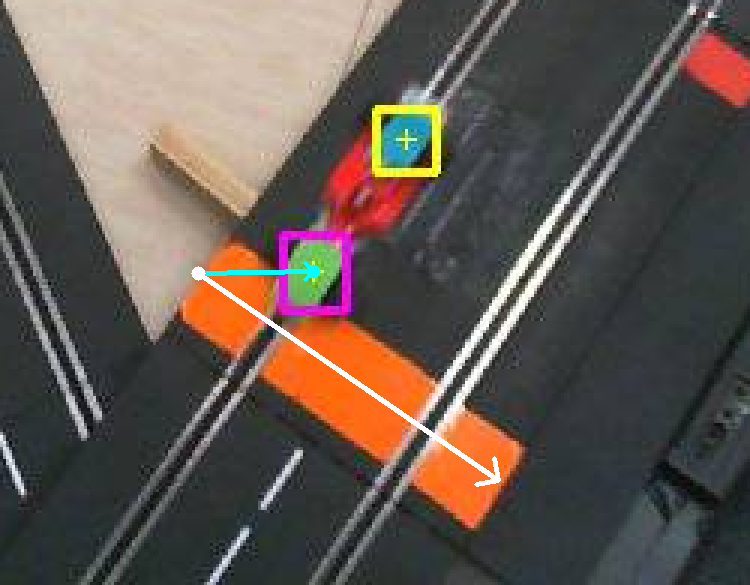
\includegraphics[width=\textwidth]{imaxes/IMPLEMENTACION/meta_vector_a_antes.png}
        \caption{Antes de cruzar}
        \label{fig:producto-vectorial-a}
    \end{subfigure}
    \hfill
    \begin{subfigure}[b]{0.48\textwidth}
        \centering
        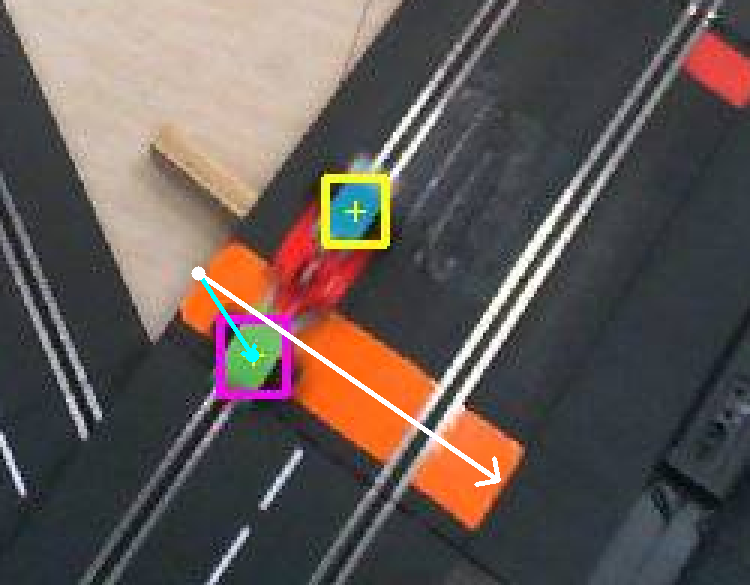
\includegraphics[width=\textwidth]{imaxes/IMPLEMENTACION/meta_vector_b_despues.png}
        \caption{Después de cruzar}
        \label{fig:producto-vectorial-b}
    \end{subfigure}
    \caption{Cambio de signo del producto vectorial al cruzar la línea de meta.}
    \label{fig:producto-vectorial}
\end{figure}

El método arrastra una limitación que ya señalaba Mario López~\cite{tfgmario}: el signo se calcula contra la recta infinita que contiene al segmento y, como el circuito es cerrado, esa recta vuelve a cortar la pista en otro punto, donde el signo cambia igual. Él lo evitaba exigiendo que el coche estuviese a menos de vez y media su longitud de un extremo de la meta; aquí el cambio de signo se ignora mientras la distancia de la pegatina al segmento supere un umbral configurable. Esta solución sustituye además a la de Adrián Rego~\cite{tfgadrian}, que fue la primera que se implementó y que fallaba la cuenta con el coche muy lento o detenido sobre la línea, mientras que el cambio de signo no depende de la velocidad a la que se cruce.

En cada cruce el controlador publica el tiempo y el número de vuelta en su \emph{topic} de telemetría y notifica el evento a todas las instancias del algoritmo, indicando si la vuelta fue limpia. Esto ocurre igual cuando el coche lo conduce una persona: en modo manual el controlador calibra, recibe posiciones, cuenta vueltas y publica telemetría exactamente igual, y lo único que no hace es publicar consigna, de forma que el puente nunca toca ese carril. Sirve para registrar una carrera conducida por una persona con el mismo formato de datos que una automática y poder compararlas después con la herramienta de análisis (sección~\ref{subsec:visualizacion-analisis}).
\label{subsec:control-automatico-manual}

\section{Implementación del algoritmo de velocidad}
\label{sec:implementacion-algoritmo}

El algoritmo diseñado en la sección~\ref{sec:algoritmo-arquitectura} recibe una posición del coche sobre la imagen de una cámara y devuelve el valor de PWM que hay que aplicar al carril, o bien la indicación de descartar el fotograma, en cuyo caso el controlador mantiene el último valor válido. Todo lo que decide sale de la trayectoria aprendida durante la calibración y de la desviación que el coche muestra respecto a ella.

\subsection{Instancias por cámara}
\label{subsec:algoritmo-instancias}

El algoritmo no trabaja sobre el circuito completo, sino sobre la porción que observa una cámara: cada lista de puntos del diccionario del controlador da lugar a una instancia independiente, con su propia cadena de celdas, sus propias zonas y su propio perfil de PWM. No existe, por tanto, una trayectoria global ni un sistema de referencia común, y ninguna instancia sabe nada de las demás; el único punto del proyecto donde todas se llevan a un plano común es la herramienta de análisis en diferido (sección~\ref{subsec:visualizacion-analisis}), que queda fuera del lazo de control. La alternativa, fusionar las trayectorias en un mapa único, exigiría calibrar la posición relativa de las cámaras y aportaría poco a un control que solo necesita saber dónde está el coche dentro del tramo que se está viendo.

La visión de conjunto la aporta el controlador, que enruta cada posición a la instancia de la cámara que la originó según el campo \texttt{camara\_id} del mensaje (sección~\ref{subsec:mensajes-propios}), decide qué cámara está activa, cierra un derrape en una y abre su continuación en la siguiente, propaga hacia atrás las reducciones que no caben en una porción y determina si una vuelta ha sido limpia en todo el trazado. Esos mecanismos se describen en la sección~\ref{subsec:algoritmo-coordinacion}.

\subsection{Cadena de celdas y localización del coche}
\label{subsec:algoritmo-celdas}
\label{subsec:algoritmo-localizacion}

La trayectoria base (sección~\ref{subsec:trayectoria-base}) se transforma en una sucesión ordenada de celdas equiespaciadas. El remuestreo es necesario porque los puntos crudos no están repartidos de forma uniforme: su separación depende de la velocidad que llevase el coche al grabarlos y de si todas las posiciones enviadas por la cámara llegaron al controlador. Se recorre la trayectoria colocando una celda cada cierta distancia fija e interpolando entre puntos consecutivos, de modo que las celdas quedan repartidas sobre el recorrido real con independencia de cómo cayeran los puntos originales. Los saltos que superan un umbral reciben otro tratamiento, porque corresponden a tramos que la cámara no ve —un puente, un túnel— y dentro de ellos no hay nada que interpolar: se crea una única \emph{celda gigante} que registra la longitud real del hueco y que se trata entera con un mismo valor de PWM, sin poder localizar el coche ni detectar derrapes en su interior.

Sobre esa cadena se sitúan las dos pegatinas. Para cada una se busca la celda más próxima al centroide y después se proyecta el centroide sobre los dos segmentos que unen esa celda con la anterior y la posterior, conservando la menor de las dos distancias; la proyección hace falta porque medir contra el punto de la celda daría una distancia dependiente de dónde caiga la celda, mientras que contra los segmentos se obtiene la distancia perpendicular a la trayectoria. Por eso tampoco puede proyectarse a través de una celda gigante, donde no hay trayectoria conocida sobre la que hacerlo. Cada distancia tiene después un uso distinto: la de la delantera es una comprobación de que el coche sigue el recorrido esperado, y si supera un umbral la detección se considera inválida y el fotograma se descarta sin calcular PWM; la de la trasera es la señal con la que se detectan los derrapes.

\subsection{Detección de derrapes}
\label{subsec:algoritmo-derrapes}

La arquitectura exige una señal capaz de indicar en qué punto del circuito el coche ha perdido el control (sección~\ref{subsec:derrape-arquitectura}), y la escogida es esa distancia perpendicular de la pegatina trasera: cuando la parte trasera del coche se abre, la distancia crece mientras la delantera sigue marcando la posición sobre el trazado. La detección es una máquina de estados que se alimenta en cada fotograma con la celda y la distancia de la trasera: al superarse el umbral se abre un derrape y se anota su celda inicial, mientras se mantenga por encima se prolonga actualizando la final, y al caer por debajo se cierra. No se abren derrapes junto a los extremos de la cadena ni junto a las celdas gigantes, donde la medida no es fiable.

La figura~\ref{fig:secuencia-derrape} recoge un caso real. Con el coche alineado la pegatina trasera va sobre el carril y su distancia es casi nula; al abrirse la parte trasera la distancia crece hasta superar el umbral, que es lo que abre el derrape, y en el instante más violento el coche queda atravesado y no se detecta ninguna de las dos pegatinas, situación que resuelve la readquisición de la sección~\ref{subsec:readquisicion}.

\begin{figure}[tbp]
    \centering
    \begin{subfigure}[b]{0.48\textwidth}
        \centering
        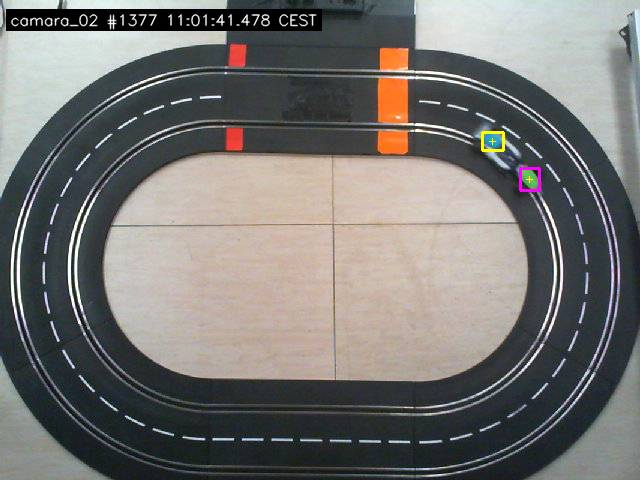
\includegraphics[width=\textwidth]{imaxes/IMPLEMENTACION/derrape_seq_a_antes.png}
        \caption{Coche alineado con el carril}
        \label{fig:secuencia-derrape-a}
    \end{subfigure}
    \hfill
    \begin{subfigure}[b]{0.48\textwidth}
        \centering
        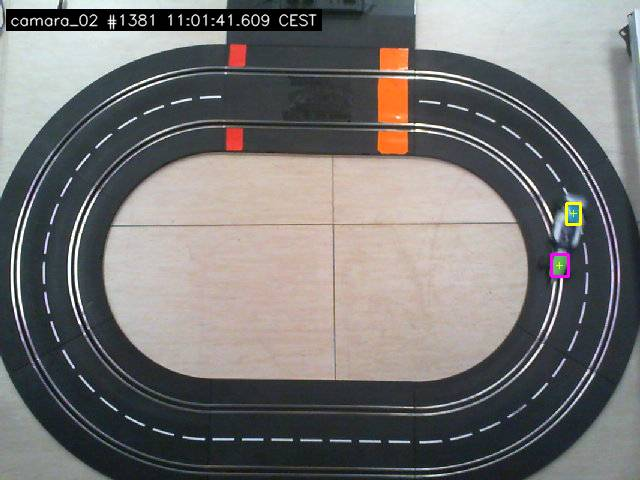
\includegraphics[width=\textwidth]{imaxes/IMPLEMENTACION/derrape_seq_b_inicio.png}
        \caption{La parte trasera empieza a abrirse}
        \label{fig:secuencia-derrape-b}
    \end{subfigure}

    \vspace{0.7em}
    \begin{subfigure}[b]{0.48\textwidth}
        \centering
        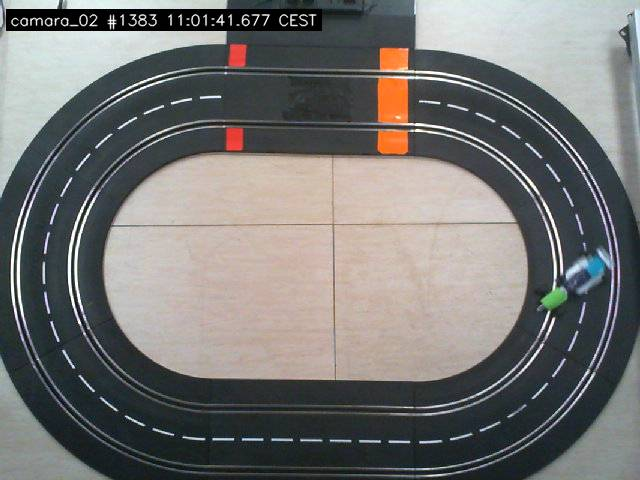
\includegraphics[width=\textwidth]{imaxes/IMPLEMENTACION/derrape_seq_c_completo.png}
        \caption{Derrape completo, sin detección}
        \label{fig:secuencia-derrape-c}
    \end{subfigure}
    \hfill
    \begin{subfigure}[b]{0.48\textwidth}
        \centering
        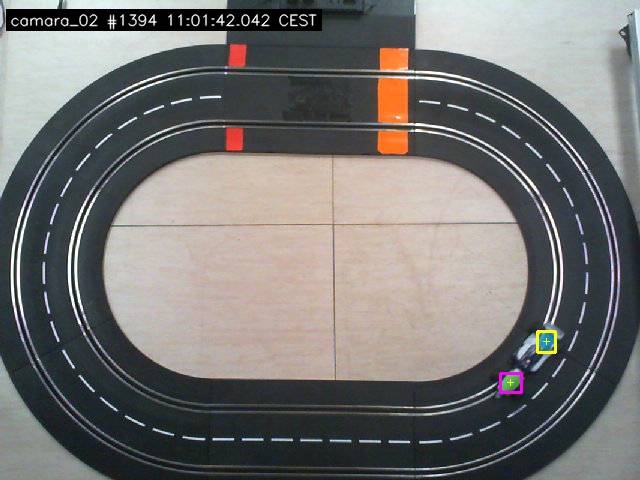
\includegraphics[width=\textwidth]{imaxes/IMPLEMENTACION/derrape_seq_d_recuperado.png}
        \caption{Seguimiento readquirido}
        \label{fig:secuencia-derrape-d}
    \end{subfigure}
    \caption{Secuencia de un derrape en el circuito con forma de óvalo.}
    \label{fig:secuencia-derrape}
\end{figure}

\subsection{Castigo de zonas y ciclo de aprendizaje}
\label{subsec:algoritmo-aprendizaje}

Cada instancia mantiene la partición de su cadena en zonas y aplica sobre ellas las dos políticas definidas en la sección~\ref{subsec:zonas-politicas}. El castigo se dispara al cerrarse un derrape: su intervalo de celdas se extiende hacia atrás una distancia fija en píxeles, que es el tramo de anticipación que exige la arquitectura, y el resultado se convierte en una zona de derrape cuyo PWM es el mínimo de los de las zonas que cubría el intervalo menos una reducción fija de dos unidades, con \texttt{minimum\_speed} como suelo. Si el derrape cae dentro o junto a una zona de derrape ya existente ambas se fusionan, y en ese caso el retroceso añadido es menor que el de una zona nueva, porque la existente ya aplicó el suyo al crearse; si cada reincidencia retrocediera la distancia completa, las zonas protegidas acabarían cubriendo el circuito entero y el perfil no volvería a subir en ningún tramo. Las celdas gigantes alcanzadas por un derrape o por su retroceso se castigan como una unidad, ya que dentro del hueco no hay precisión para distinguir una parte de otra.

La mejora se dispara con el paso por meta. El controlador comprueba si hubo algún derrape en alguna cámara durante la vuelta y comunica el resultado a todas las instancias; cada zona sin derrape sube su PWM en una unidad, con \texttt{maximum\_speed} como techo, salvo las que registraron uno en las últimas vueltas, que permanecen protegidas durante un número configurable de vueltas antes de poder volver a subir.

Las figuras~\ref{fig:derrape-trazas} y~\ref{fig:derrape-dist} recorren el ciclo completo sobre tres vueltas consecutivas de una sesión real. En la vuelta~21 la trasera va pegada a la trayectoria base, la distancia nunca se acerca al umbral y el PWM se mantiene constante en todo el recorrido, con una única zona. En la~22 la trasera se abre en la curva y la distancia supera el umbral durante diez fotogramas, lo que cierra un derrape y castiga la zona. En la~23 el perfil ya trae el PWM rebajado en ese tramo, visible como un escalón, y el coche vuelve a pasar limpio.

\begin{figure}[tbp]
    \centering
    \begin{subfigure}[b]{0.48\textwidth}
        \centering
        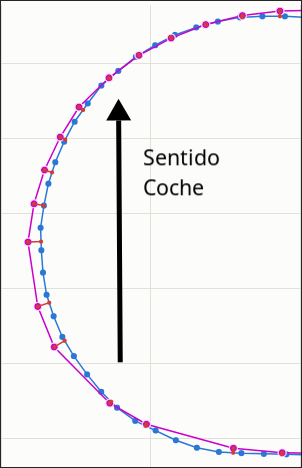
\includegraphics[width=\textwidth]{imaxes/IMPLEMENTACION/derrape_traza_v21.png}
        \caption{Vuelta 21, limpia}
        \label{fig:derrape-trazas-a}
    \end{subfigure}
    \hfill
    \begin{subfigure}[b]{0.48\textwidth}
        \centering
        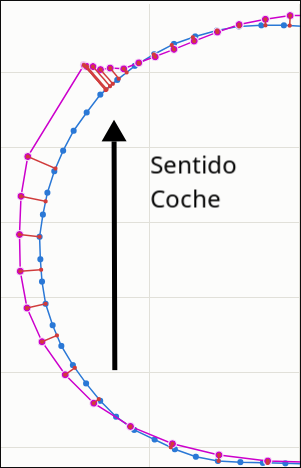
\includegraphics[width=\textwidth]{imaxes/IMPLEMENTACION/derrape_traza_v22.png}
        \caption{Vuelta 22, con derrape}
        \label{fig:derrape-trazas-b}
    \end{subfigure}

    \vspace{0.7em}
    \begin{subfigure}[b]{0.48\textwidth}
        \centering
        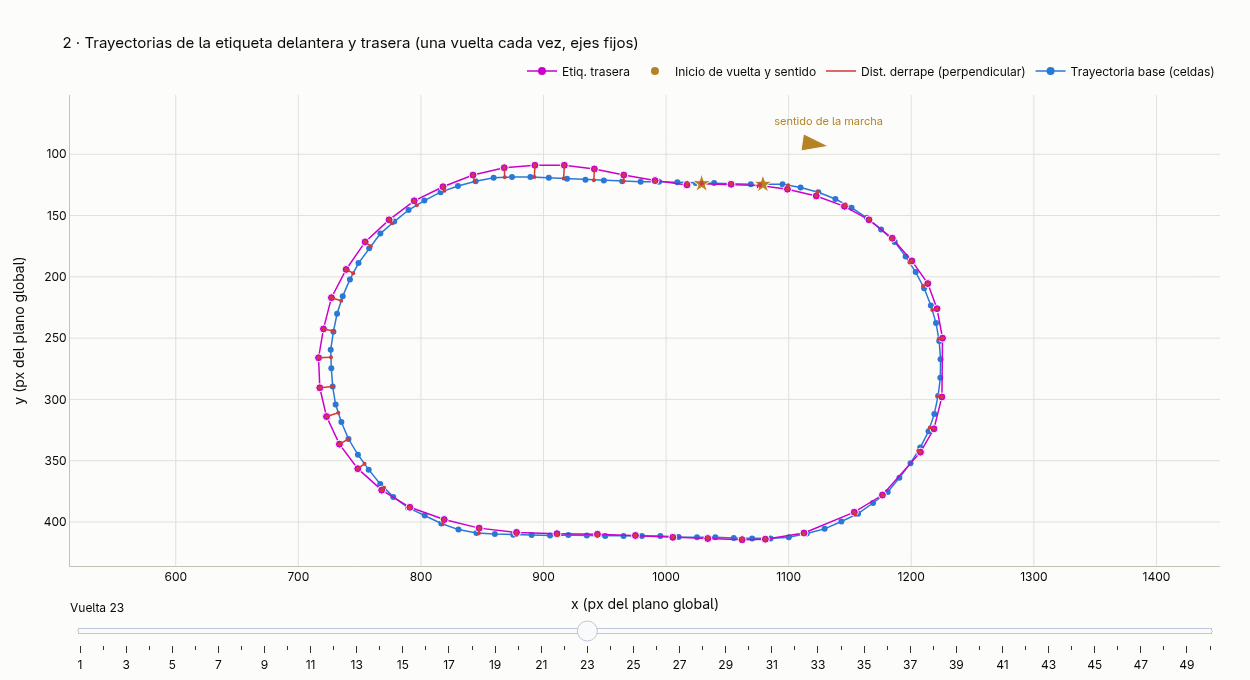
\includegraphics[width=\textwidth]{imaxes/IMPLEMENTACION/derrape_traza_v23.png}
        \caption{Vuelta 23, ya castigada}
        \label{fig:derrape-trazas-c}
    \end{subfigure}
    \caption{Recorrido de la pegatina trasera (magenta) frente a la trayectoria base (azul) en tres vueltas consecutivas. Los segmentos rojos son la distancia perpendicular que mide el algoritmo.}
    \label{fig:derrape-trazas}
\end{figure}

\begin{figure}[p]
    \centering
    \begin{subfigure}[b]{0.85\textwidth}
        \centering
        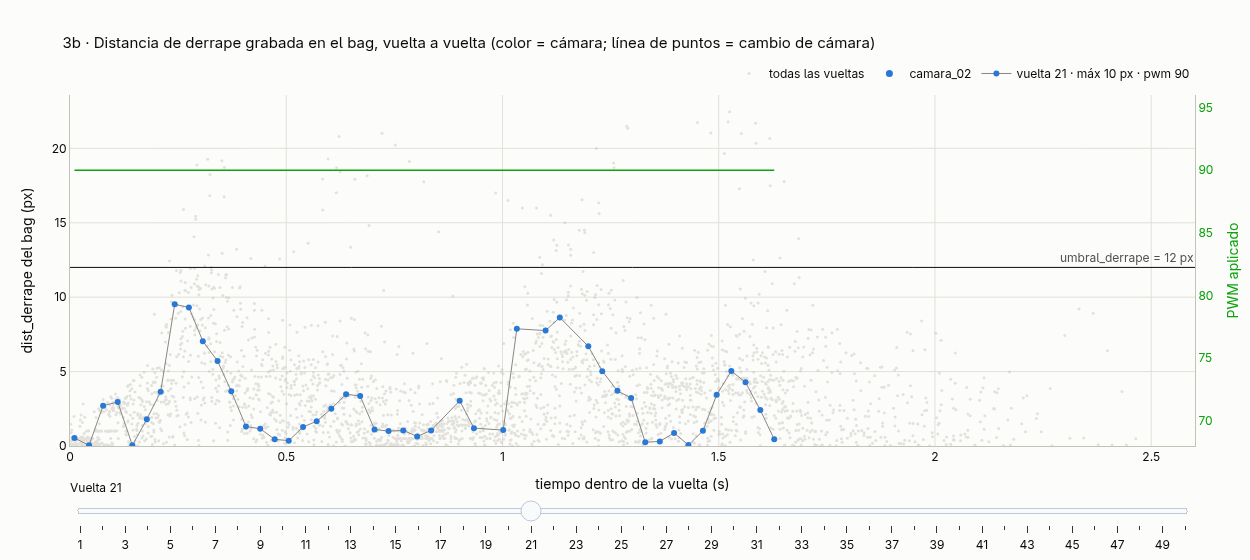
\includegraphics[width=\textwidth]{imaxes/IMPLEMENTACION/derrape_dist_v21.png}
        \caption{Vuelta 21}
        \label{fig:derrape-dist-a}
    \end{subfigure}

    \vspace{0.5em}
    \begin{subfigure}[b]{0.85\textwidth}
        \centering
        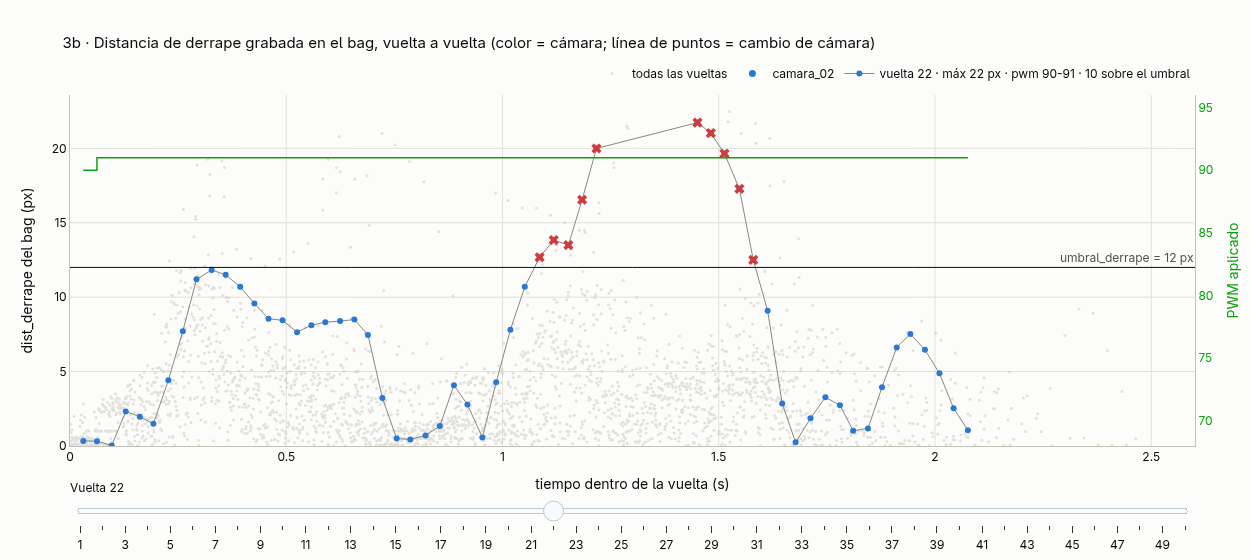
\includegraphics[width=\textwidth]{imaxes/IMPLEMENTACION/derrape_dist_v22.png}
        \caption{Vuelta 22}
        \label{fig:derrape-dist-b}
    \end{subfigure}

    \vspace{0.5em}
    \begin{subfigure}[b]{0.85\textwidth}
        \centering
        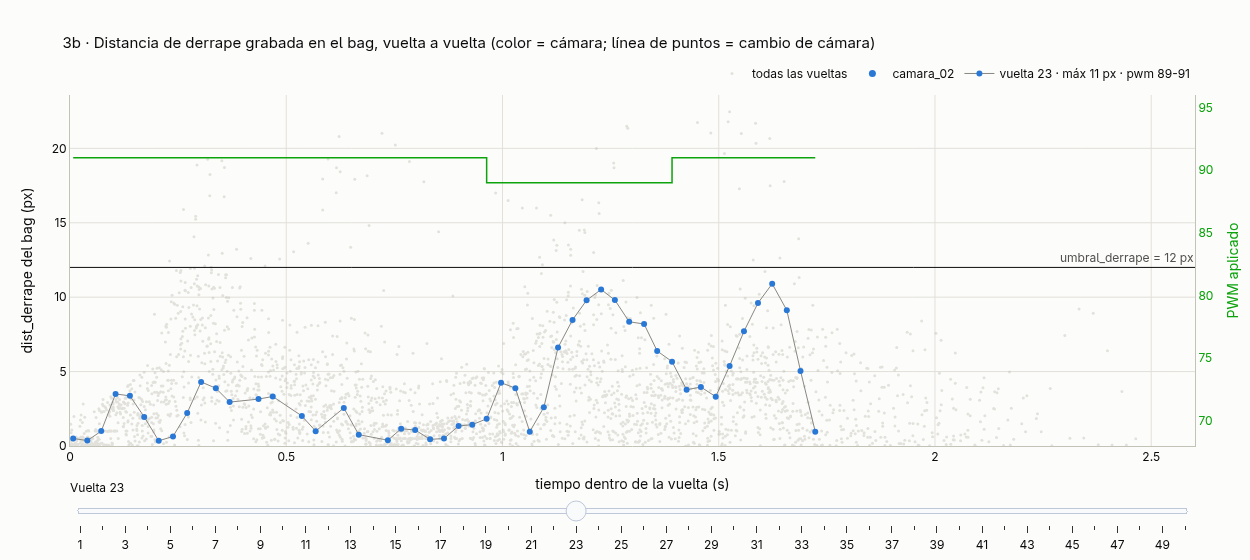
\includegraphics[width=\textwidth]{imaxes/IMPLEMENTACION/derrape_dist_v23.png}
        \caption{Vuelta 23}
        \label{fig:derrape-dist-c}
    \end{subfigure}
    \caption{Distancia de la pegatina trasera a lo largo de cada vuelta (eje izquierdo) frente al PWM aplicado (línea verde, eje derecho). Las aspas rojas marcan las muestras que superan el umbral y abren el derrape. El escalón verde de la vuelta~23 es la zona creada por el castigo de la anterior.}
    \label{fig:derrape-dist}
\end{figure}

\subsection{Coordinación entre cámaras}
\label{subsec:algoritmo-coordinacion}

Como cada instancia conoce solo su porción del circuito, hay tres situaciones que ninguna puede resolver sola y que asume el controlador.

La primera es la transición del coche entre cámaras. Cuando dos campos de visión se solapan ambas publican posiciones intercaladas del mismo coche, así que la cámara activa se mantiene mientras siga entregando fotogramas válidos y solo se cambia cuando deja de hacerlo durante un breve intervalo y otra sí está entregando. En cada cambio el controlador notifica la pérdida de visión a la cámara saliente y anota el relevo; como el coche recorre siempre el circuito en el mismo sentido, tras una vuelta completa ese registro contiene el orden secuencial de las cámaras, aprendido en carrera y sin ninguna configuración manual.

La segunda es el derrape repartido entre dos cámaras. Al recibir la notificación de pérdida de visión la instancia saliente cierra el derrape que tuviera abierto y, si seguía activo, la entrante recibe la orden de abrir uno nuevo, de modo que la zona se extiende entre cámaras y el derrape se detecta aunque el corte caiga en mitad de una curva.

La tercera es la propagación de reducciones, que ocurre cuando un derrape se produce cerca del inicio de la porción visible de una cámara, algo habitual si una curva queda repartida entre dos. El retroceso del castigo se sale por el inicio antes de agotarse y los píxeles restantes corresponden a un tramo de otra cámara, así que la instancia anota ese sobrante como reducción pendiente; el controlador lo recoge y, según el orden aprendido, ordena a la cámara precedente que lo aplique al final de su trayectoria, creando o ampliando allí la zona de derrape. Esa reducción externa no incrementa el contador de derrapes de quien la recibe, porque ya lo contabilizó la cámara que lo observó, pero la zona queda igualmente protegida. Si tampoco cupiera en la trayectoria de la cámara anterior, el sobrante volvería a quedar pendiente y seguiría propagándose hacia atrás hasta agotarse.

\section{Actuación sobre el circuito}
\label{sec:sistema-actuacion}
\label{subsec:actuacion-topics}

El nodo puente es puramente consumidor: no publica nada, se limita a suscribirse a los \emph{topics} en los que cada controlador anuncia el PWM de su carril, con una suscripción por coche declarado en la configuración. De cada mensaje extrae el carril y el valor, y le aplica dos comprobaciones antes de mandarlo al puerto serie. La primera es un filtro de repetición: el nodo guarda el último valor enviado a cada carril y descarta el mensaje si coincide. Como los controladores publican una consigna por cada posición recibida y el PWM se mantiene estable durante tramos enteros del circuito, este filtro reduce drásticamente el tráfico sobre el puerto, que es el punto más lento de la cadena. La segunda es una validación del rango admitido por el hardware, entre 0 y 255, como última barrera frente a consignas mal formadas.

El puente se suscribe también al \emph{topic} de calibración de cada coche autónomo, porque durante esa fase es él quien aplica al carril una potencia constante que da la velocidad de calibración: los controladores todavía no publican consigna alguna. En cuanto un coche cierra su vuelta, el puente pasa a aplicar el valor que publica su controlador. Los carriles de los coches marcados como manuales no se tocan en ningún momento.
\label{subsec:actuacion-interfaz}

Por debajo, la comunicación con la placa se encapsula, como en el trabajo de Adrián Rego~\cite{tfgadrian}, en una clase que abstrae el puerto serie en operaciones de alto nivel —fijar la velocidad de un carril, la de ambos o detenerlos— y que se comunica con un protocolo textual mínimo. El envío es bloqueante: la interfaz espera la confirmación de la placa antes de dar la orden por completada, y ese carácter bloqueante es precisamente lo que serializa el acceso al único puerto disponible. Tanto esa interfaz como el montaje electrónico y el \emph{firmware} de la placa se reutilizan sin cambios de ese trabajo, funcionan tal cual y se describen en el anexo~\ref{anexo:hardware}. Lo que este trabajo aporta no es el montaje, sino su encaje en la arquitectura distribuida: en el trabajo previo la interfaz vivía dentro de la misma aplicación de escritorio que procesaba las imágenes y decidía las velocidades, y aquí queda detrás de un nodo que centraliza y ordena el acceso desde toda la red.

\section{Grabación y análisis en diferido}
\label{sec:sistema-visualizacion}

La visualización se resuelve con dos herramientas independientes que solo se comunican a través de los ficheros que una genera y la otra consume (figura~\ref{fig:flujo-visualizacion}). La de grabación se despliega junto al resto del sistema y almacena todo lo que circula por la red mientras la sesión está en marcha; la de análisis se ejecuta después, si el usuario quiere, y construye a partir de esa grabación un \emph{dashboard} web para estudiar la carrera vuelta a vuelta.

\begin{figure}[H]
    \centering
    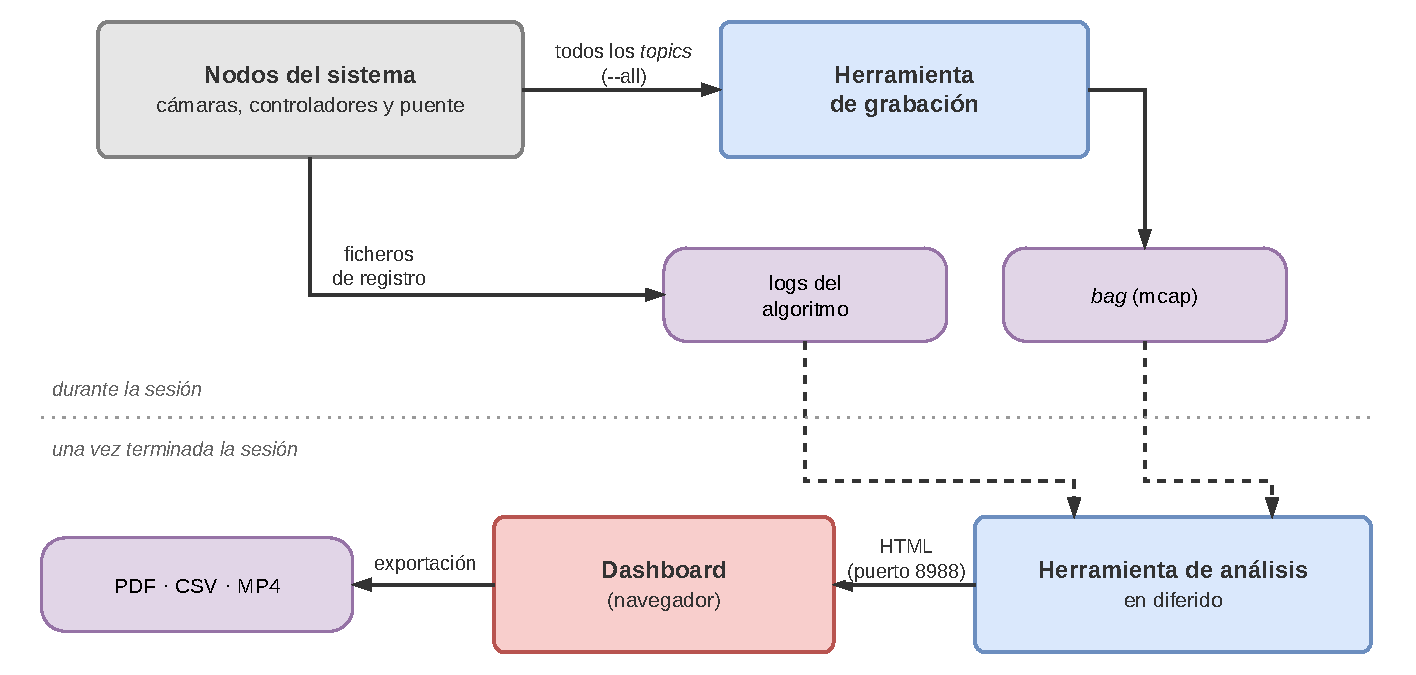
\includegraphics[width=\textwidth]{imaxes/IMPLEMENTACION/flujo_analisis_sistema.pdf}
    \caption{Flujo de datos entre la grabación de la sesión y el análisis en diferido.}
    \label{fig:flujo-visualizacion}
\end{figure}

\subsection{Herramienta de grabación}
\label{subsec:visualizacion-grabacion}

La grabación se construye sobre \emph{rosbag2} (sección~\ref{sec:ros2-rosbag}), empaquetada en un contenedor junto con las definiciones de los mensajes propios, que hay que compilar dentro para poder interpretarlos. Su cometido es capturar sin pérdidas todo el tráfico de la red y dejarlo en disco, sin procesar ni interpretar nada.

La primera versión trabajaba con una lista explícita de \emph{topics}, construida a partir del número de cámaras y de coches configurados, y resultó una fuente constante de errores, porque cada \emph{topic} nuevo o renombrado había que acordarse de reflejarlo en ella. La versión definitiva graba la totalidad de los \emph{topics} y sondea periódicamente en busca de otros, suscribiéndose a los que van apareciendo, con lo que no impone ningún orden de arranque; la calidad de servicio se resuelve igual, adaptando el perfil de cada suscripción al que ofrecen los publicadores que encuentra en lugar de mantener un fichero que reprodujese las políticas del sistema. Se escogió el formato \emph{mcap} porque lleva embebida la definición de cada mensaje, de modo que un \emph{bag} sigue siendo legible aunque las definiciones hayan cambiado desde que se grabó, algo que ocurrió varias veces conforme avanzaba el proyecto.

\subsection{Herramienta de análisis en diferido}
\label{subsec:visualizacion-analisis}

El análisis cruza dos fuentes: la grabación, de la que obtiene todo lo que se publicó en la red, y los ficheros de \emph{log} que escribe el algoritmo, de los que obtiene su estado interno. La primera describe qué hizo el coche y los segundos explican por qué el sistema decidió lo que decidió, de manera que solo cruzándolas puede relacionarse un comportamiento con la decisión que lo provocó.

El resultado es una página web autocontenida con gráficas interactivas, organizada en las secciones que recoge el cuadro~\ref{tab:secciones-dashboard}, desde la que pueden exportarse las gráficas en PDF, los datos en CSV y un vídeo que combina las imágenes de todas las cámaras. Como cada cámara trabaja en sus propias coordenadas de imagen, las gráficas espaciales se dibujan sobre un plano global común aplicando a cada una una traslación fija; este es el único punto del sistema donde las trayectorias de las distintas cámaras se llevan a un mismo plano, y puede hacerse porque queda fuera del lazo de control. La herramienta se ejecuta también en un contenedor, que a diferencia del resto no forma parte del sistema desplegado: se levanta bajo demanda indicándole qué sesión analizar, sirve el \emph{dashboard} en un puerto accesible desde el anfitrión y termina al pararlo. Necesita contenedor por la misma razón que la grabación, porque leer ficheros \emph{mcap} exige tener disponibles las bibliotecas de ROS~2 y las definiciones de los mensajes.

\begin{table}[htbp]
\centering
\resizebox{\textwidth}{!}{
\begin{tabular}{|c|l|}
\hline
\rowcolor{ArqAzulClaro}
\textbf{Sección} & \textbf{Contenido} \\
\hline
0 & Resumen de la sesión \\
\hline
1 & Valor del derrape en cada punto del recorrido (3D) \\
\hline
2 & Trayectorias de las etiquetas delantera y trasera \\
\hline
3 & Distancia de derrape de la etiqueta trasera \\
\hline
4 & Mapa del circuito con el PWM de cada celda \\
\hline
5 & Tiempos por vuelta \\
\hline
6 & Evolución de las zonas, perfil de PWM y resumen por vuelta \\
\hline
7 & Visor de las imágenes grabadas y generación de vídeo \\
\hline
8 & Descarga de los datos en formato CSV \\
\hline
\end{tabular}
}
\caption{Secciones del \emph{dashboard} generado por la herramienta de análisis.}
\label{tab:secciones-dashboard}
\end{table}